%%***********************************************
%% Plantilla para TFG.
%% Escuela Técnica Superior de Ingenieros Informáticos. UPM.
%%***********************************************

%%-----------------------------------------------
%% Importar Preámbulo:
% -*-coding: utf-8 -*-
%%***********************************************
%% Plantilla para TFG.
%% Escuela Técnica Superior de Ingenieros Informáticos. UPM.
%%***********************************************
%% Preámbulo del documento.
%%***********************************************
\documentclass[a4paper,11pt]{book}
\usepackage[utf8]{inputenc}
\usepackage[T1]{fontenc}
\usepackage[english,spanish,es-lcroman]{babel}
\usepackage{bookman}
\decimalpoint
\usepackage{graphicx}
\usepackage{amsfonts,amsgen,amsmath,amssymb}
\usepackage[top=3cm, bottom=3cm, right=2.54cm, left=2.54cm]{geometry}
\usepackage{afterpage}
\usepackage{colortbl,longtable}
\usepackage[pdfborder={0 0 0}]{hyperref} 
\usepackage{pdfpages}
\usepackage{url}
\usepackage[stable]{footmisc}
\usepackage{parskip} % para separar párrafos con espacio.
\usepackage{acronym}
%%-----------------------------------------------
\usepackage{fancyhdr}
\pagestyle{fancy}
\fancyhf{}
\fancyhead[LO]{\leftmark}
\fancyhead[RE]{\rightmark}
\setlength{\headheight}{1.5\headheight}
\cfoot{\thepage}

\addto\captionsspanish{ \renewcommand{\contentsname}
  {Tabla de contenidos} }
\setcounter{tocdepth}{4}
\setcounter{secnumdepth}{4}

\renewcommand{\chaptermark}[1]{\markboth{\textbf{#1}}{}}
\renewcommand{\sectionmark}[1]{\markright{\textbf{\thesection. #1}}}
\newcommand{\HRule}{\rule{\linewidth}{0.5mm}}
\newcommand{\bigrule}{\titlerule[0.5mm]}

\usepackage{appendix}
\renewcommand{\appendixname}{Anexos}
\renewcommand{\appendixtocname}{Anexos}
%\renewcommand{\appendixpagename}{Anexos}
%%-----------------------------------------------
%% Páginas en blanco sin cabecera:
%%-----------------------------------------------
\usepackage{dcolumn}
\newcolumntype{.}{D{.}{\esperiod}{-1}}
\makeatletter
\addto\shorthandsspanish{\let\esperiod\es@period@code}

\def\clearpage{
  \ifvmode
    \ifnum \@dbltopnum =\m@ne
      \ifdim \pagetotal <\topskip
        \hbox{}
      \fi
    \fi
  \fi
  \newpage
  \thispagestyle{empty}
  \write\m@ne{}
  \vbox{}
  \penalty -\@Mi
}
\makeatother
%%-----------------------------------------------
%% Estilos código de lenguajes: Consola, C, C++ y Python
%%-----------------------------------------------
\usepackage{color}

\definecolor{gray97}{gray}{.97}
\definecolor{gray75}{gray}{.75}
\definecolor{gray45}{gray}{.45}

\usepackage{listings}
\lstset{ frame=Ltb,
     framerule=0pt,
     aboveskip=0.5cm,
     framextopmargin=3pt,
     framexbottommargin=3pt,
     framexleftmargin=0.4cm,
     framesep=0pt,
     rulesep=.4pt,
     backgroundcolor=\color{gray97},
     rulesepcolor=\color{black},
     %
     stringstyle=\ttfamily,
     showstringspaces = false,
     basicstyle=\scriptsize\ttfamily,
     commentstyle=\color{gray45},
     keywordstyle=\bfseries,
     %
     numbers=left,
     numbersep=6pt,
     numberstyle=\tiny,
     numberfirstline = false,
     breaklines=true,
   }
\lstnewenvironment{listing}[1][]
   {\lstset{#1}\pagebreak[0]}{\pagebreak[0]}

\lstdefinestyle{consola}
   {basicstyle=\scriptsize\bf\ttfamily,
    backgroundcolor=\color{gray75},    
    }

\lstdefinestyle{CodigoC}
   {basicstyle=\scriptsize,
	frame=single,
	language=C,
	numbers=left
   }
   
\lstdefinestyle{CodigoC++}
   {basicstyle=\small,
	frame=single,
	backgroundcolor=\color{gray75},
	language=C++,
	numbers=left
   }

\lstdefinestyle{Python}
   {language=Python,    
   }
\makeatother   
%%-----------------------------------------------
%% Cargar datos relativos al TFG:
%% (actualizar estos datos en secciones/_DatosTFG.tex) 
%%***********************************************
%% Plantilla para TFG.
%% Escuela Técnica Superior de Ingenieros Informáticos. UPM.
%%***********************************************
%% Información requerida para completar la portada.
%%*********************************************** 

%% Escribe Nombre y Apellidos del autor del trabajo:
\newcommand{\NombreAutor}{ Marcos Pino Gamazo }

%% Escribe el Grado: 
\newcommand{\Grado}{ Grado en Ingeniería Informática }

%% Escribe el Título del Trabajo:
\newcommand{\TituloTFG}{ Desarrollo de un Chatbot para Público Infantil para Clasificar Sonidos del Cielo. Versión 2} 

%% Escribe Nombre y Apellidos del Tutor del trabajo: 
\newcommand{\NombreTutor}{ Raquel Cedazo León } 

% Escribe el Departamento al que pertenece el Tutor:
\newcommand{\Departamento}{ Ingeniería Eléctrica, Electrónica Automática y Física Aplicada }

% Escribe la fecha de lectura, en formato: Mes - Año
\newcommand{\Fecha}{ <<Febrero  2021>> }
%%***********************************************


%%-----------------------------------------------
%% Documento:
\begin{document}
%%***********************************************
%% Plantilla para TFG.
%% Escuela Técnica Superior de Ingenieros Informáticos. UPM.
%%***********************************************
%% Portada. 
%%***********************************************
\begin{titlepage}

\begin{minipage}{0.15\linewidth}
\hspace*{-2.5cm}
\noindent

\includegraphics[scale=0.5]{include/EscUpm.png} \qquad\qquad
\end{minipage}
\begin{minipage}{0.7\linewidth}
\begin{center}
\huge{ Universidad Politécnica\\de Madrid }\\
\vspace*{0.5cm}
\Large{\textbf{Escuela Técnica Superior de \\
Ingenieros Informáticos}}
\end{center}
\end{minipage}
\begin{minipage}{0.2\linewidth}

\includegraphics[scale=0.5]{include/FacInformatica.png} 
\end{minipage}

\vspace*{1cm}
\begin{center}
\Large{Grado en  \Grado{} }
\end{center}

\vspace*{1cm}
\begin{center}
\huge{ Trabajo Fin de Grado }
\end{center}

\vspace*{0.5cm}
\begin{center}
\huge\bfseries {  \TituloTFG{} } 
\end{center}

\vspace*{5cm}

\noindent
\large{Autor: \NombreAutor{} }\\
\large{Tutor(a): \NombreTutor{} }


\vspace*{4cm}
\begin{center}
Madrid, \Fecha
\end{center}

%%--------------------------------
\newpage
\thispagestyle{empty}
%%--------------------------------
\noindent
Este Trabajo Fin de Grado se ha depositado en la ETSI Informáticos de la Universidad Politécnica de Madrid para su defensa.

\vspace*{4cm}
\noindent
\textit{Trabajo Fin de Grado}\\
\textit{Grado en} \Grado{}

\begin{enumerate}
\item[\textit{Título:}] \textbf{\TituloTFG{}}
\end{enumerate}
\Fecha


\vspace*{3cm}

\noindent
\begin{tabular}{ll}
\textit{Autor:} & \NombreAutor{}  \\ 
\textit{Tutor:} & \NombreTutor{}  \\ 
                & \Departamento{} \\
                & ETSI Informáticos\\
                & Universidad Politécnica de Madrid
\end{tabular} 

\end{titlepage}


%%-----------------------------------------------
%% Numeración romana:
\frontmatter
%%-----------------------------------------------
\chapter*{Resumen}

Este Trabajo Final de Grado tiene como misión el diseño y desarrollo de una aplicación cuya principal funcionalidad es, la clasificación de  meteoros mediante sonidos generados por ordenador a partir de detecciones llevadas a cabo mediante radiofrecuencia. 

El proyecto Sonidos del Cielo tiene como objetivo hacer accesible la ciencia a personas con discapacidad visual y para ello, se pretende desarrollar una herramienta mediante la cual se pueda seguir una conversación en \textit{lenguaje natural}, estas herramientas se conocen por el término en inglés \textit{chatbot}. Será necesario que la herramienta sea capaz de reconocer la voz y a su vez transmitir mediante voz la información generada por la aplicación. Esto va a facilitar el acceso a la herramienta no sólo a personas con problemas de visión sino también a niños que aún no sepan leer o escribir.

El diseño completo del proyecto requiere del diseño y desarrollo estructural tanto de una bases de datos en las que se almacenen los elementos necesarios para el proyecto (sonidos de meteoros, curvas de luz, espectrograma, parámetros de detección, etc) como de una API Rest que sirva como controlador y ofrezca servicios entre la base de datos y el chatbot y futuras herramientas que puedan requerirla.

Además, se ha desarrollado una versión preliminar del chatbot para realizar las pruebas necesarias sobre la API Rest y así consolidar las tecnologías y servicios a utilizar en el proyecto Sonidos del Cielo.


%Hasta ahora, se ha realizado el diseño y volcado de la base de datos antigua que contenía la información de las radio detecciones, y se ha comenzado la creación de un API Rest para conectar la base de datos con la aplicación.

%Además, se han mantenido reuniones semanales entre todos los miembros del proyecto, así como la confección de los documentos intermedios y finales del trabajo.


%%--------------
\newpage
%%--------------

\chapter*{Abstract}

The objetive of this Final Degree Project is the design and development an application whose principal funcionality is the classification of meteors using computer-generated sounds from meteor echoes detected by radio frequency.

The Sonidos del Cielo project aims to make science accesible to people with visual disabilities and to achieve this, it is intended to develop a tool through wich you cna have a conversation in natural language, these tools are known as chatbots for the union of the words chat and robot.

It will be necesary for the tool to be able to recognize the voice and at the same time transmit de information generated by the chatbot by voice, wich will facilitate access to the tool not only for people with visual disabilities but also for children who still can't read or write.

The complete design of the project requires the design and structural development of a database in wich all the necessary elements for the project are stores (meteor sounds, light curves, spectrograms, detection parameters, etc) and a REST API that will be used as a controller and will offered services between the database and the chatbot and future tools that may require it.

In addition, a preliminary version of the chatbot has been developed to carry out the necessary test on the REST API and thus consolidate the technologies and services to be used in the Sonidos del Cielo project.


%%%%%%%%%%%%%%%%%%%%%%%%%%%%%%%%%%%%%%%%%%%%%%%%%%%%%%%%%%%
%% Final del resumen. 
%%%%%%%%%%%%%%%%%%%%%%%%%%%%%%%%%%%%%%%%%%%%%%%%%%%%%%%%%%%
\tableofcontents
\listoffigures

%%-----------------------------------------------
%% Numeración arábiga:
\mainmatter
%%----------------------------------------------- 
\input{secciones/01_Introduccion}
\chapter{Estado del Arte}

\section{Bases de Datos}
\subsection{Historia de las bases de datos}

Hay que remontarse un poco atrás en el tiempo, concretamente hasta 1880 cuando Herman Hollerith desarrolló una máquina para procesar los datos más rápido de lo que los humanos podían hacerlo. Desarrolló unas tarjetas perforadas mediante las cuales podía realizar un censo de la población completa de Estados Unidos en solo dos años, algo que en esa época era poco más que una quimera. Aun así, la primera vez que se tiene conocimiento del uso del término bases de datos fue en el año 1963 en un simposio celebrado en California y se refiere a ella como un conjunto de información relacionada y que tiene cierta estructura.

Los primeros modelos que fueron desarrollados fueron bases de datos jerárquicas y en red, pero rápidamente se vio que estaban muy limitadas técnicamente y eran demasiado simples. Posteriormente, IBM revolucionó el sector en la década de los 70 creando el modelo relacional de base de datos, mucho más potente y muy bien adoptada por el mundo laboral.
En los 2000 empezaron a aparecer proyectos de código libre que supusieron una competencia en un sector liderado siempre por sistemas privados (IBM y Oracle), entre los más usados destacan MySQL y PostgreSQL. La tendencia a la utilización de sistemas NoSQL contribuyó al detrimento de los sistemas de bases de datos de las grandes empresas. \cite{sanchez2016historia} 

\subsection{Tipos de Bases de Datos}
\subsubsection{Bases de Datos Jerárquicas}

Se trata del modelo más antiguo, se ha visto superado por el modelo relacional. El lenguaje de marcado XML utiliza este tipo de modelo para almacenar los datos. El sistema más conocido es el IMS/DB creado por IBM.

\begin{figure}[h]
    \centering
    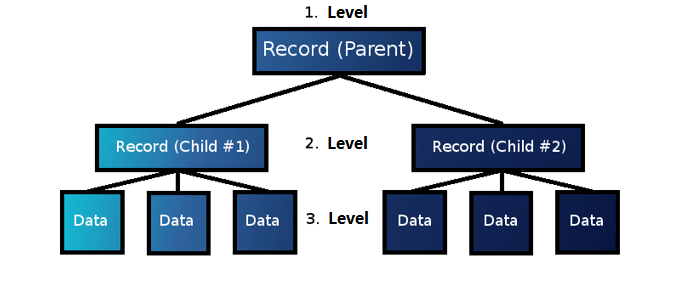
\includegraphics[scale=0.4]{{include/figuras/Jerarquico.png}}
    \caption{Modelo jerárquico}
    \label{fig:bd_jerarquica}
\end{figure}

En este tipo de modelo, cada registro sólo posee un precedente excepto la raíz, formando una estructura arbolada como la que se puede ver en la figura \ref{fig:bd_jerarquica}. En este tipo de modelo, los hijos sólo pueden tener un padre pero un padre puede tener múltiples hijos. Dada esta relación estricta, los niveles que no tengan una relación directa, no pueden interactuar entre ellos y realizar una conexión entre varios árboles tampoco es sencillo. Por este motivo, estas estructuras son consideradas inflexibles aunque por otro lado son muy fáciles de comprender.

\subsubsection{Bases de Datos en Red}

Se desarrolló de manera concurrente al relacional pero con el tiempo se vería superado. No revelan relaciones padre-hijo estrictas sino que cada registro puede tener múltiples precedentes, lo que genera una estructura en red y de ahí su nombre. 
\begin{figure}[h]
    \centering
    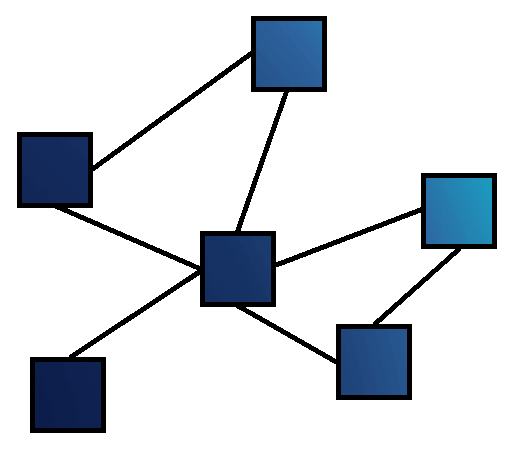
\includegraphics[scale=0.3]{{include/figuras/ModeloEnRed.png}}
    \caption{Modelo de red}
    \label{fig:bd_red}
\end{figure}

Al registro central se tiene acceso desde los otros cinco y desde él, puede accederse a otros cinco registros. En este modelo pueden definirse dependencias, de forma que si accedes al registro superior necesitas pasar por el central para poder alcanzar el registro de la derecha. Hoy en día este modelo de bases de datos se suele utilizar en algunos supercomputadores. Algunos de los modelos más conocidos son el UDS de Siemens y el DMS de Sperry Univac.

\subsubsection{Bases de Datos Relacionales}

Es el modelo más utilizado en la actualidad y es considerado como el estándar de la industria. Normalmente utiliza el lenguaje SQL y se trata de un modelo basado en tablas. Para definir las relaciones se utiliza álgebra relacional y gracias a esta se puede hallar la información de las diferentes relaciones como se puede ver en la figura \ref{fig:bd_relacional}.

\begin{figure}[h]
    \centering
    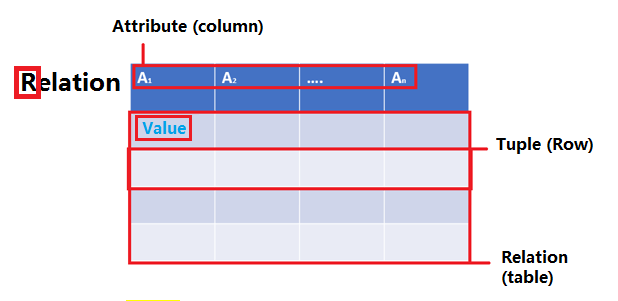
\includegraphics[scale=0.5]{{include/figuras/Relacional.png}}
    \caption{Modelo relacional}
    \label{fig:bd_relacional}
\end{figure}

El modelo relacional funciona mediante tablas independientes que determinan la organización de los datos y sus conexiones. Para poder identificar sin problema un registro es necesario establecer una \textbf{clave primaria}, que habitualmente se trata del primer atributo y no se puede modificar.

\subsubsection{Modelo de Base de Datos Orientado a Objetos}

Surgen a finales de 1980 y a día de hoy han tenido una aplicación muy minoritaria. Este tipo de bases de datos suelen utilizarse en plataformas de lenguajes Java y .NET. La más conocida es \textit{db4o} y destaca por su bajo consumo de memoria. Utilizan un lenguaje OQL, muy parecido a SQL.

\begin{figure}[h]
    \centering
    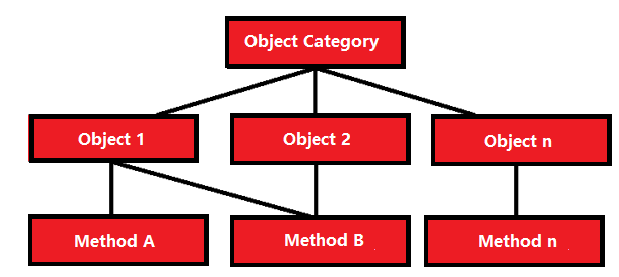
\includegraphics[scale=0.4]{{include/figuras/Objetos.png}}
    \caption{Modelo orientado a objetos}
    \label{fig:bd_objetos}
\end{figure}

En este modelo los datos se almacenan en objetos además de las funciones y los atributos que los definen. Los objetos pueden ser complejos y estar formados por múltiples tipos de datos; se identifican por un identificador de objeto único y se agrupan en clases al igual que en lenguaje de programación orientado a objetos, creando una jerarquía de clases.

\subsubsection{Modelo de Base de Datos Orientado a Documentos}

En este modelo, la unidad mínima de almacenamiento de datos es el documento pero no se deben confundir con los documentos que se generan mediante un procesador de texto. En estos documentos los datos se almacenan como \textbf{pares claves-valor}, como no tienen una definición, los documentos que forman este tipo de bases de datos son muy diferentes entre sí. Cada documento es una unidad cerrada entre sí y establecer relaciones entre documentos no es una tarea sencilla, aunque por otro lado, en este tipo de bases de datos no es necesario establece relaciones.

\begin{figure}[h]
    \centering
    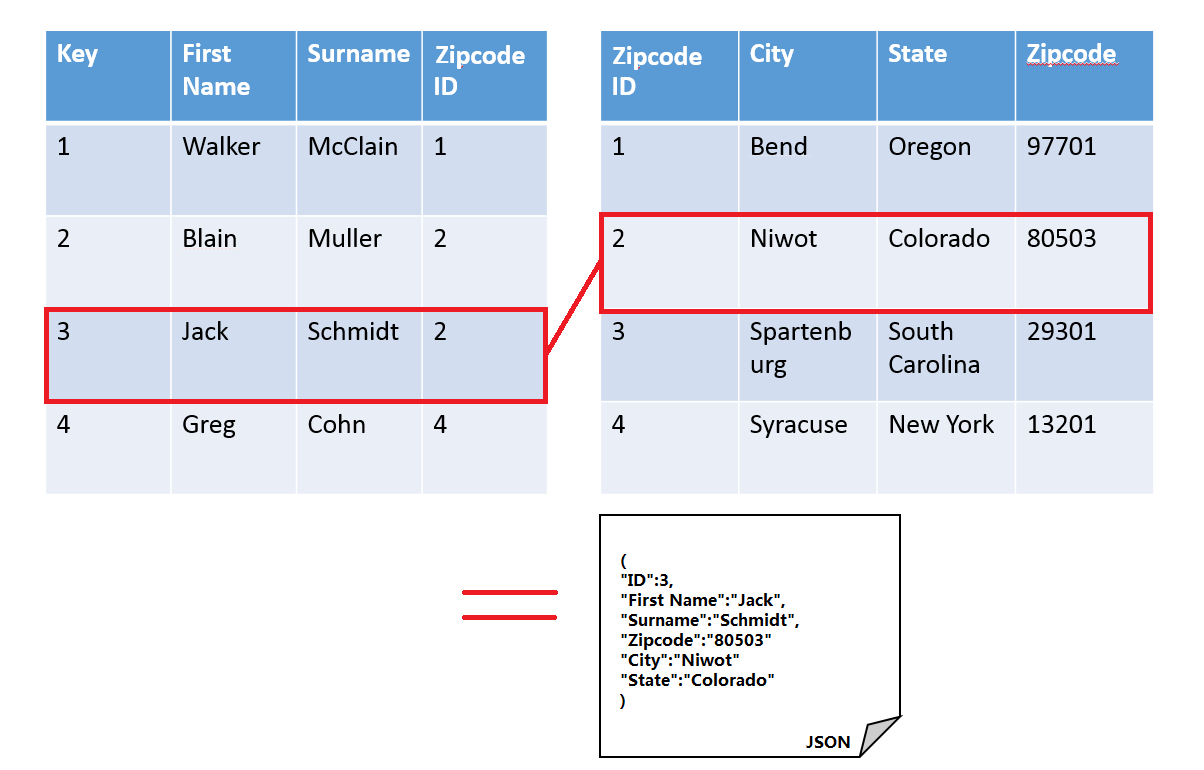
\includegraphics[scale=0.25]{{include/figuras/OrientadaDocumentos.png}}
    \caption{Modelo orientado a documentos}
    \label{fig:bd_documentos}
\end{figure}

La idea fundamental de este tipo de modelos es que los datos que tienen relación se guardan en un mismo documento, esto provoca que el número de consultas a la base de datos sea mucho menor que en una base de datos relacional. Son muy útiles para aplicaciones web debido a que puede almacenarse formularios HTML. Con el avance de la web 2.0 estas bases de datos aumentaron exponencialmente su popularidad y son utilizadas hoy en día por plataformas como Google, Facebook, Twitter, Amazon, etc.


\section{Asistentes Virtuales}

\subsection{Historia de los Chatbots}

Un chatbot es una aplicación de software capaz de mantener una conversación con un usuario dando una serie de respuestas automáticas, establecidas con anterioridad a diferentes entradas que pueda dar el usuario. Existen distintas teorías sobre el origen de los chatbots. 

La primera de ellas, defiende que en la década de 1950, el matemático inglés Alan Turing investigó si una máquina sería capaz de imitar las respuestas de un humano mediante el análisis de una conversación de texto entre un humano y una máquina. 

La segunda, más extendida, sitúa el origen en el año 1966 en el Instituto Tecnológico de Massachusetts (MIT), allí el profesor de informática Joseph Weizenbaum desarrolló en el laboratorio de inteligencia artificial el programa \textit{Eliza}, el concepto es que actuara como si se tratase de un terapeuta. Funcionaba de la siguiente manera: examinaba palabras clave que tenía el enunciado del emisor para poder responder con una serie de oraciones que tenía previamente registradas.

En 1972, surgió el chatbot \textit{Parry}, que simulaba ser una persona con esquizofrenia paranoide. A diferencia de Eliza disponía de una estrategia de comunicación cimentada en premisas y ''respuestas emocionales'' en base a las interacciones con los usuarios. \cite{StreamGenerator}

Como detalle curioso, Eliza y Parry fueron puestos a conversar entre sí mediante la red ARPANET \footnote{ARPANET: red de ordenadores creada por el Departamento de Defensa de los Estados Unidos para conectar varias instituciones académicas y estatales.}  
Posteriormente fue desarrollado \textit{Jabberwacky} por el programador inglés Rollo Carpenter, capaz de mantener una conversación mediante la voz. Aunque fue terminado en 1981 no fue hasta 1997 cuando fue publicado online.
A partir del año 2006 han surgido una gran cantidad de chatbots entre los que cabe destacar:

IBM Watson, nombrado así por el primer director ejecutivo de IBM. En un principio fue desarrollado para responder preguntas y respuestas ideadas por humanos para el concurso Jeopardy. El concurso es el típico de preguntas y respuestas solo que las preguntas son formuladas mediante juegos de palabras y giros lingüisticos. Se presentó al concurso en 2011 por primera vez y fue capaz de ganar a dos especialistas. A partir de ese instante, ha pasado por varias adaptaciones utilizando procesamiento de lenguaje natural y machine learning\footnote{Machine Learning: disciplina dentro de la Inteligencia Artificial que crea sistemas y software capaces de aprender automáticamente} para procesar una gran cantidad de datos. En 2013, IBM anunció que Watson podía ser utilizado para la toma de decisiones en el tratamiento del cáncer de pulmón. 

Tal vez el chatbot más conocido mundialmente sea el asistente virtual desarrollado por Apple, \textit{Siri}. Utiliza consultas dadas mediante comandos de voz para ayudar al usuario de diversas formas, realizar tareas, recordatorios, búsquedas y modificar configuraciones del sistema.

De este mismo estilo tenemos los chatbot \textit{Alexa} creado por Amazon,\textit{Cortana} desarrollado por Microsoft y \textit{Google Now} desarrollado por Google.


\begin{figure}[H]
    \centering
    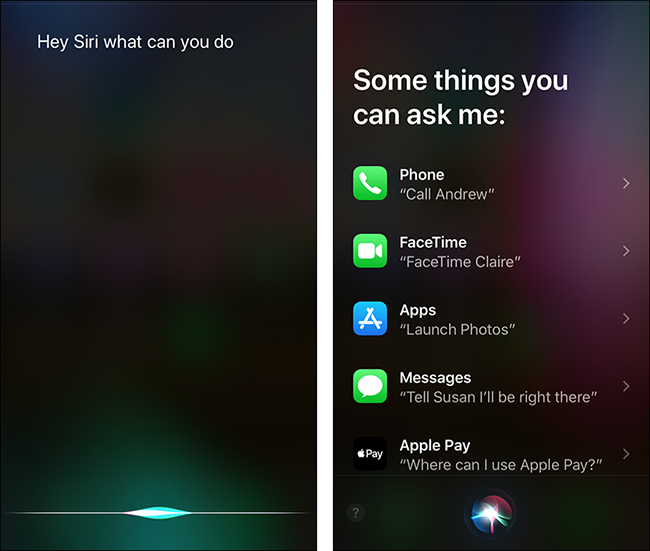
\includegraphics[scale=0.4]{{include/figuras/siri.png}}
    \caption{Interfaz de Siri}
    \label{fig:siri_gui}
\end{figure}

La utilización de estos asistentes ha crecido exponencialmente debido a la necesidad de dar servicios a los clientes, sin importar la hora ni el lugar ya que están siempre disponibles cuando el usuario lo necesite.
Hoy en día se están implementando cada vez más en servicios de mensajería instantánea para la transmisión de noticias, las más destacables son Telegram, Slack, Whatsapp, Discord, Skype, Kik y WeChat

\begin{figure}[h]
    \centering
    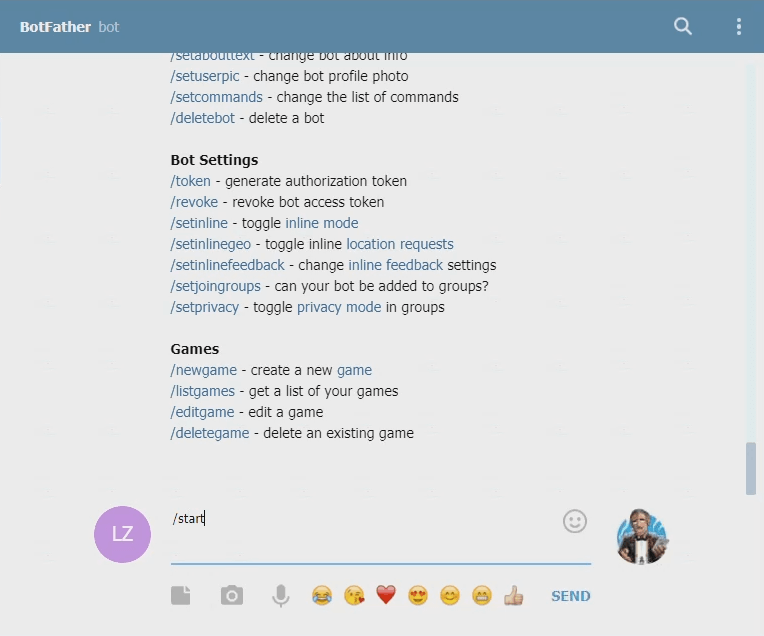
\includegraphics[width=0.5\textwidth]{include/figuras/BotFather.png}
    \caption{Telegram BotFather}
    \label{fig:telegram}
\end{figure}
Alguna de estas aplicaciones han desarrollado servicios mediante los cuales puedes crear nuevos bots sin tener que programar una sola linea de código, como puede ser BotFather de Telegram. Así como tiendas con búsquedas y sistemas de valoraciones para aumentar el uso de estas aplicaciones. 

\subsection{Frameworks}

Un framework es un tipo de estructura con una serie de archivos y pautas que se utiliza para desarrollar proyectos con una estructura y metodología, es decir, algo así como una plantilla que simplifica la creación de una solución.

\subsubsection{DialogFlow}
Framework de desarrollo de chatbots creado en 2010 y mantenido por Google\cite{Dialogflow}. Es capaz de comprender el lenguaje natural y nos brinda herramientas para la fabricación de diálogos y la recreación de conversaciones. Destaca por la gran cantidad de interfaces de conversación en los que se puede desplegar (Google home, google assistant, wereables, teléfonos, coches). Tiene soporte para más de 14 idiomas y es capaz de resolver abreviaturas y funcionar con faltas de ortografía. 
Posee una interfaz muy intuitiva y permite crear chatbots en una cantidad pequeña de tiempo. 

\begin{figure}[H]
    \centering
    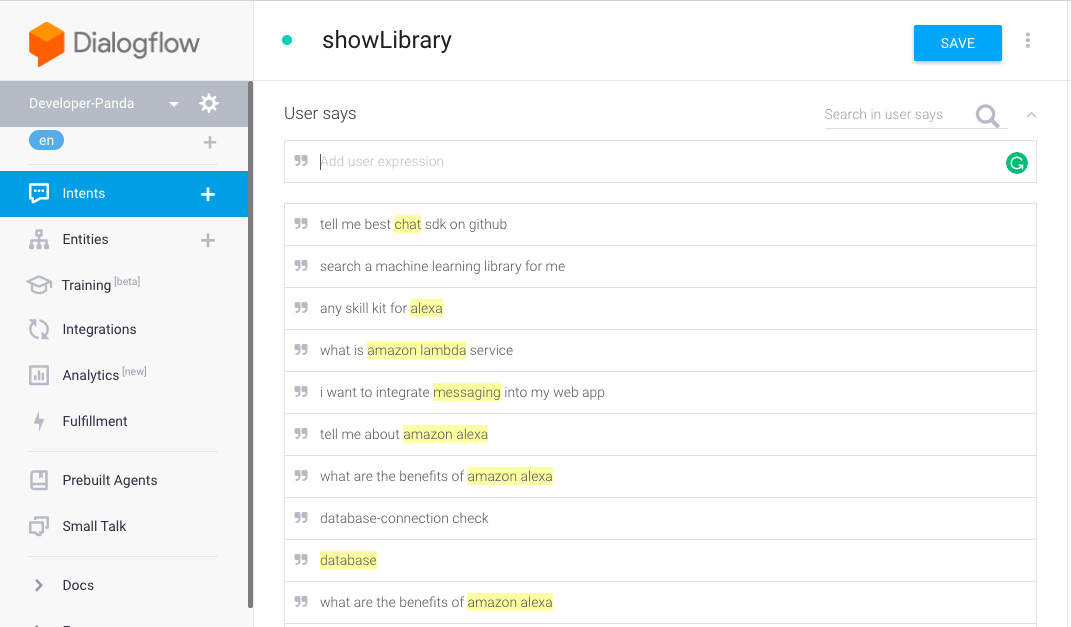
\includegraphics[scale=0.4]{{include/figuras/DialogFlow.png}}
    \caption{Interfaz de dialogflow}
    \label{fig:dialogflow_gui}
\end{figure}


\subsubsection{Microsoft Bot Framework}
Desarrollado por Microsoft, crea chatbots rapidamente a través de la herramienta Microsoft Bot Builder y los conecta con Azure Bot Service, lo que nos permite una rápida creación del bot ya que nos proporciona diversas plantillas para seleccionar cuando se está creando el bot y nos brinda todas las mejoras de la nube creada por Microsoft. Puede editarse con directamente desde la página web usando el editor de Azure o algún IDE de desarrollo como Visual Studio o Visual Studio Code \cite{MicrosoftBotBuilder}. Posee su propio sistema de procesamiento natural del lenguaje llamado LUIS (\textit{Language Understanding Intelligent Service}).  




\subsubsection{IBM Watson}
Creado por IBM, es capaz de comprender y responder a las preguntas de los usuarios mediante lenguaje natural \cite{MicrosoftBotBuilder}. Watson está compuesto actualmente por un clúster de al menos 750 servidores \textit{IBM Power 750}, con unos 16 TB de memoria RAM, lo que proporciona una potencia de cálculo bruto de unos \textbf{80 Petalops}, convirtiéndolo así en uno de los supercomputadores más potentes del mundo. 

\subsubsection{Amazon Lex}
Creado y gestionado por Amazon, permite establecer comuncicaciones con todos sus productos Eco y con su asistente virtual Alexa. Es una de las mejores herramientas en cuanto a conversión de voz a texto. Con esta herramienta se pueden crear bots con un lenguaje natural sofisticado. A diferencia de los anteriores, tiene una interfaz más intuitiva para principiantes aunque por el contrario, dispone de menos herramientas, aunque posee todas las necesarias en un chatbot.

\subsubsection{Rasa}
Por último cabe destacar Rasa, una framework \textit{Open Source} de Machine Learning que nos permite crear conexiones entre las máquinas y el usuario. Posee herramientas para entender al usuario mediante el componente Rasa NLU (Natural Langugage Understanding), generar el diálogo con Rasa NLG (Natural Language Generation) y un motor (Rasa Core) capaz de definir cuál será la siguiente acción a tomar en función del mensaje transmitido por el usuario.   


\subsection{Librerías}

Una librería es uno o varios archivos escritos en algún tipo de lenguaje de programación, que proporcionan varias funcionalidades. Al contrario que un framework, una librería no establece la estructura sobre cómo debe realizarse el desarrollo, sino que da funcionalidades genéricas que han sido programadas con anterioridad y evitan que haya que escribir código de más, aumentando la calidad del código y reduciendo el tiempo de desarrollo.
Vamos a analizar las librerías existentes más importantes para el lenguaje de programación Python, debido a que se trata de un lenguaje simple, elegante ordenado, portable y que requiere de pocas líneas de código para generar programas completos.

\subsubsection{Chatterbot}
Se trata de una librería de Machine Learning basada en las conversaciones y diálogos tradicionales. Está diseñada de manera independiente al idioma, por lo que se puede entrenar en cualquier lenguaje que está asegurado su correcto funcionamiento. 
El Machine Learning implementado en Chatterbot consigue que mediante la interactuación con los humanos permite que mejore su propio conocimiento. También es posible implementarlo junto a otras librerías para añadir funcionalidad como Text to Speech \footnote{Text to Speech: por sus siglas en inglés TTS, procedimiento de síntesis mediante el cual se transforma el texto escrito en voz.}

Es también compatible con librerías para aportar más funcionalidades como puede ser la conversión de texto a voz y así poder interactuar con el usuario sin necesidad de escribir.

\subsubsection{Natural Language ToolKit} NTLK por sus siglas en inglés, se trata de una plataforma para crear chatbots con lenguaje humano. Dispone de funcionalidades muy interesantes desde el punto de vista del reconocimiento del lenguage como la tokenización , derivación, etiquetado, análisis y razonamiento semántico.

\subsubsection{ChatbotAI} Nos permite crear un chatbot con muy pocas líneas de código. Genera un controlador del chat y bots con inteligencia artificial que permiten una integración muy sencilla con API Rest. Esta inteligencia artificial nos genera múltiples características como aprender, memorizar, manejar conversaciones según el tema \cite{chatbotAI}. 

\subsubsection{Tensorflow} Es uan plataforma de código abierto gestionada por Google. Se trata de una biblioteca de aprendizaje automático con la que es posible construir y entrenar redes neuronales para detectar patrones y correlaciones en el aprendizaje y razonamiento de los humanos. Tiene diversas formas de interacción con el usuario (interfaces web, API Rest, interfaces gráficas de usuario, y líneas de comandos).

\subsection{Procesamiento de Lenguaje Natural}
Una de las partes más importantes de un asistente virtual es el Natural Lenguage Processinng (NLP), gracias a esta herramienta, el programa es capaz de entender la forma en la que nos expresamos los humanos. 
El procesamiento del lenguaje natural es una rama de la inteligencia artificial la cual se encarga de analizar y estudiar las interacciones en lenguaje natural entre los humanos y los ordenadores. Este campo posee varias funciones atrayentes.

\begin{itemize}
    \item \textbf{Comprensión del lenguaje natural}: mediante esta función el programa consigue analizar lo que dice el usuario y comprender el mensaje. Para ello es estrictamente necesario que exista una base de datos del lenguaje en el que queremos que se exprese el chatbot de manera que pueda comprender la gramática, la semántica y el vocabulario del lenguaje que queremos que domine.
    \item \textbf{Recuperación de la información}: esta parte es la encargada de extraer las palabras claves del texto proporcionado.
    \item \textbf{Generación del lenguaje natural}: capacidad de dar respuestas a los mensajes enviados en lenguaje natural. Esta parte del programa se encarga de escoger las posibles respuestas y establecer un orden para que la respuesta proporcionada sea la más indicada y correcta gramaticalmente.
    \item \textbf{Reconocimiento y síntesis del lenguaje hablado}: hace que el chatbot sea capaz de transformar las respuestas que se le entregan mediante el habla y transformarlas a texto para su tratamiento. Una vez la respuesta del chatbot se genere, el módulo se encargará de convertirla a voz.
    \item \textbf{Detección de emociones y sentimientos}: hay ciertos programas que a través del estudio del lenguaje de las entradas que da el usuario son capaces de detectar los sentimientos y emociones.
\end{itemize}

\subsection{Ventajas e Inconvenientes de Utilizar Chatbots en un Entorno Profesional}
El afloramiento de los asistentes virtuales ha permitido la mejora y la automatización de procesos y servicios dentro del entorno profesional pero al no tener todas las habilidades que posee un humano, su utilización también posee ciertos inconvenientes.

\subsubsection{Ventajas}

\begin{itemize}
    \item Disponibilidad: un chatbot una vez implementado puede funcionar 24 horas al día 7 días a la semana.
    \item Reducción de costes: puesto que es capaz de responder las preguntas más frecuentes y realizar las tareas más solicitadas no será necesario tener asistentes humanos, permitiendo una reducción de costes y su posible utilización en otros campos más necesarios.
    \item Auto-aprendizaje: posee algún tipo de inteligencia artificial es capaz de aprender nuevos comportamientos a través de las interacciones con los clientes así como nuevos comportamientos que no hayan sido programados. 
    \item Eficiencia: Un asistente humano tiene una capacidad limitada de atención en un rango de tiempo mientras que el asistente puede tener tantas instancias como sea necesario.
\end{itemize}



\subsubsection{Inconvenientes}

\begin{itemize}
    \item Inteligencia: aunque tenga implementado inteligencia artificial, un asistente no es más inteligente que un humano y hay veces que no entiende el mensaje que el usuario le entrega y puede provocar un atasco del proceso. Esto puede llevar a que si el usuario pierde la paciencia, no se complete el proceso de compra.
    \item Tiempo: es necesario emplear tiempo en entrenar al asistente.
    \item Toma de decisiones: un chatbot no es capaz de decidir en base a lo que se haya enseñado con anterioridad.
    \item Coste: es cierto que la implementación de un chatbot permite reducir los costes de mano de obra aunque si bien es cierto que en un primer momento el coste de implementarlo puede ser mayor puesto que hay que programarlo de tal manera que se adapte al campo de la empresa, es decir, hay que especializarlo.
\end{itemize}


\subsection{Principales Aplicaciones de los Chatbots}

\subsubsection{Información}
Durante una crisis sanitaria como la que está viviendo el planeta con el virús SARS-CoV-2 la tendencia más normal es que noticias falsas o bulos se propaguen con una gran velocidad aunque cada día hay más gente que busca información y ayuda a través de recursos en línea. 

Para todos ellos, la Organización Mundial de la Salud (OMS) \cite{oms} ha desarrollado un chatbot para que las personas se mantengan informadas mediante un chatbot implementado en la aplicación de mensajería instantánea WhatsApp, ha sido diseñado de tal manera que permita dar información rápida y fiable sobre temas relacionados con el coronavirus. Se trata de un bot que funciona mediante comandos, utilizando emojis o palabras que nos indica el propio bot nos proporcionará información sobre varios temas como podemos observar en la figura \ref{fig:oms}. De momento el bot sólo esta disponible en inglés aunque está en estudio el ampliarlo a castellano, árabe, chino, francés y ruso.

\begin{figure}[H]
    \centering
    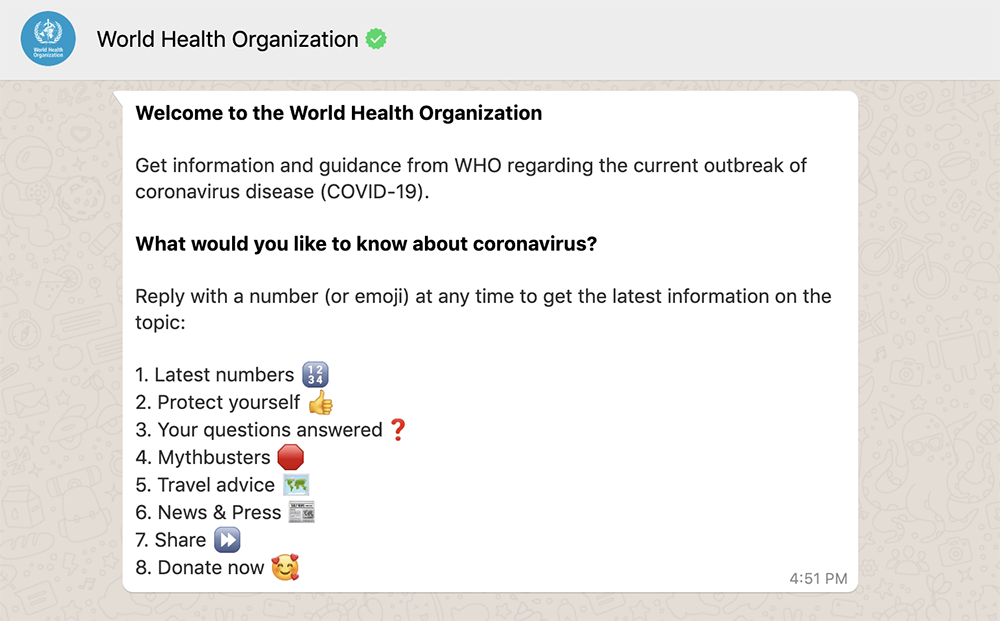
\includegraphics[scale=0.6]{include/figuras/oms.png}
    \caption{Interfaz World Health Organization}
    \label{fig:oms}
\end{figure}

\subsubsection{Salud}
En consecuencia a lo expuesto en la sección anterior, mucha gente en contraindicación de lo que aconsejan los médicos busca información sobre los síntomas que puedan padecer a través de internet. En esta línea se desarrolló Woebot \cite{woebot}, un chatbot que ayuda a reducir los síntomas de la depresión escuchando de forma activa los mensajes que envía el usuario y reaccionando a ellos con ánimo y con GIFs divertidos a mensajes positivos. Combina años de investigación en el campo de la psicología con la inteligencia artificial y el procesamiento del lenguaje natural permitiendo que se evalúe el estado emocional del usuario y guiándolo para recibir la ayuda correcta de los profesionales necesarios en el momento adecuado.

\begin{figure}[H]
    \centering
    
\includegraphics[scale=0.15]{include/figuras/woebot.jpg}
    \caption{Interfaz Woebot}
    \label{fig:woebot}
\end{figure}


\subsubsection{Viajes}
Un bot de viaje puede ahorrar una cantidad significativa de tiempo a los usuarios (organización del viaje, lugares de interés a visitar) además mediante el uso de inteligencia artificial han hecho que varias empresas del sector turísitico se lancen a la implementación de un chatbot que por un lado aumente su número de ventas y por otro reduzca la cantidad de personas necesarias para contestar a todos los usuarios con dudas.
A día de hoy, uno de los mejores chatbots de la industria es el desarrollado por KLM Royal Dutch Airlines \cite{klm}, este chatbot funciona a través de Facebook Messenger pero con la particularidad que utiliza un complemento de casilla de verificación de Facebook Messenger a la hora de realizar el pago de tal manera que capaz de proporcionar información sobre la tarjeta de embarque, el check-in y actualizaciones del estado del vuelo a través de la aplicación de mensajería instantánea.
Antes de la implementación del chatbot, KLM tenía que contestar unas 15000 conversaciones a la semana a través de las redes sociales en una docena de idiomas distintos, para poder tratar todas estas conversaciones se requiere una gran cantidad de personal y aún así existirán horarios en los cuales no se pueda conversar con el usuario. Para solucionarlo comenzaron a estudiar varias formas para prestar una atención excelente en cualquier momento del día, rápida y personalizada, como resultado llegaron a la conclusión de implementar un chatbot. 
En el primer mes de funcionamiento, el volumen de mensajes en Facebook aumentó un 40 por ciento y envió 1.7 millones de mensajes a más de 500000 clientes.

\begin{figure}[h]
    \centering
    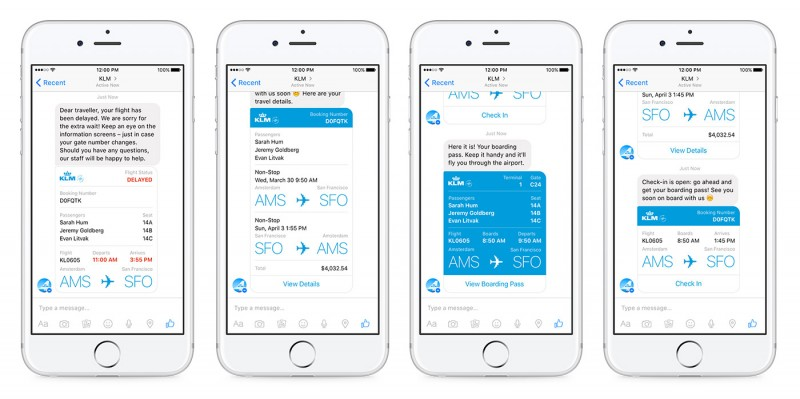
\includegraphics[width=\textwidth]{include/figuras/klm-chatbot.jpg}
    \caption{Interfaz gráfica chatbot KLM}
    \label{fig:klm}
\end{figure}


\subsubsection{Banca}
En los últimos tiempos los bancos están intentando mejorar las relaciones y la comunicación con sus clientes. Este sector tiene fama de utilizar aplicaciones y sistemas arcaicos pero cada vez son mas las entidades que buscan actualizarse y llegar a más clientes. 
El holding bancario Capital One \cite{eno} es uno de los más grandes de Estados Unidos y en 2018 lanzó su chatbot \textit{ENO}, se trata de un chatbot conversacional, es decir, es capaz de continuar una conversación y no funciona mediante comandos. Los clientes pueden mandar un sms a Eno en cualquier momento a través de la página web, la aplicación móvil del banco para comprobar transacciones recientes, el saldo o incluso para informar sobre algún problema con la tarjeta de crédito. Tiene la capacidad de incluso avisar cuando se cobra de más por una factura.

\begin{figure}[h]
    \centering
    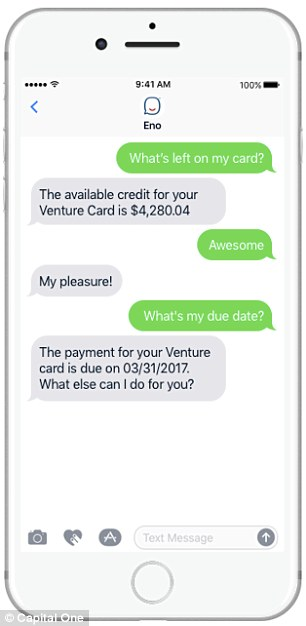
\includegraphics[scale=0.4]{include/figuras/Eno.jpg}
    \caption{Interfaz gráfica Eno}
    \label{fig:eno}
\end{figure}


En España existen algunas alternativas como por ejemplo, la aplicación imaginBank implementado por La Caixa a través de Facebook Messenger.

\subsubsection{Entretenimiento}
Los chatbots también se pueden emplear para realizar planes y lugares de ocio. Un ejemplo de esto es el asistente Mahoudrid creado por la empresa Mahou en colaboración con Ontwice basándose en la guia de ocio de nombre homónimo. 

Este asistente es capaz de recomendar locales, bares, tapas y planes. Es un bot conversacional implementado a través de Facebook Messenger mediante inteligencia artificial y te recomienda el plan perfecto en base a lo que desees tomar y tu estado de ánimo. 

\subsubsection{Restauración}
En la actualidad existen múltiples chatbots que ayudan al usuario a consultar recetas o consejos de dietética, sin embargo, el verdadero potencial de estos es el de poder recomendar restaurantes cercanos a la ubicación del usuario e incluso realizar un pedido simplemente escribiendo en un chat de mensajería instantánea y que lo tengas en tu casa en el menor tiempo posible sin tener que realizar ninguna llamada telefónica. 

Un ejemplo es el chatbot desarrollado por Burguer King \cite{burguer} e implementado en WhatsApp que se muestra en la figura \ref{fig:burguer}.


\begin{figure}[h]
    \centering
    
\includegraphics[scale=0.4]{include/figuras/BurguerKing.png}
    \caption{Chatbot Burguer King}
    \label{fig:burguer}
\end{figure}

\chapter{Desarrollo}

Para el desarrollo de este Trabajo de Fin de Grado es necesario utilizar múltiples tecnologías y herramientas. En este capítulo se explicará brevemente el estado actual de los chatbots, las distintas herramientas para desarrollarlos, así como los lenguajes de programación utilizados, qué es el procesamiento natural del lenguaje.

Lo primero que hay que tener en cuenta es que se han desarrollado tres servicios desde cero. Por un lado se ha creado una base de datos no relacional, luego una Api Rest para manejar la base de datos y por último un chatbot que será el que consuma la API y a su vez la base de datos. 

\section{Arquitectura del Proyecto}

Este Trabajo de Fin de Grado está incluido dentro de una estructura que está formada por varios proyectos que se explicarán a continuación, así como de las tecnologías seleccionadas para desarrollar el proyecto.
En el ordenador instalado en la estación de Fuenlabrada está colocado el programa \textit{Echoes Watcher} \cite{echoesWatcher}. Este programa lee el archivo de configuración  generado por Echoes para obtener datos de interés (peak, directorio, nombre estación, etc) y según se van generando ficheros de detecciones, el programa mediante un programa de monitorización, lee esos ficheros y en caso de encontrar alguna detección, se envían los datos a través de un Broker MQTT \cite{singh2015secure} al equipo ubicado en el Centro de Supercomputación y Visualización de Madrid (Cesvima).

Todos los días se procede a hacer un backup de los datos sin filtrar a otro computador del proyecto ubicado en la Escuela Técnica Superior de Ingeniería y Diseño Industrial (ESTIDI).

En el Cesvima se encuentra ubicado el programa StreamGenerator \cite{StreamGenerator}. Este programa está suscrito al broker y puede recibir datos de configuración de la estación y datos de las detecciones. Cuando recibe datos de configuración de las detecciones genera un fichero de liquidsoap \cite{liquidsoap} si no existe o si ha cambiado la configuración de la estación. Este fichero liquidsoap genera una lista de reproducción que está ubicada en el Instituto Astrofísico de Canarias y se trata de un bucle infinito de ruido (basado en el archivo de configuración) y a medida que le llegan detecciones de una estación se altera dicha lista de reproducción para añadir los sonidos generados con la detección que recibe del broker, y una vez que el sonido es reproducido, se borra. 
Por cada estación existente hay una lista de reproducción, lo que significa que existe un proceso liquidsoap ejecutándose por cada estación.  

Todos los datos existentes en la estación de Fuenlabrada pasan a través de un Pipeline gestionado mediante \textbf{Apache Airflow}. Este programa es un orquestador de servicios, es decir, es utilizado para automatizar tareas sistemáticas dividiendo estas mismas en subtareas. Los casos de uso más típicos son la automatización de carga de datos, acciones periódicas de mantenimiento y tareas de administración. Para ello permite el uso de herramientas como \textit{cron} y ejecutarlos bajo demanda.
Mediante esta herramienta se envían los datos a un servidor existente en el Departamento de Arquitectura y Tecnología de Sistemas Informáticos. En este servidor existe una base de datos relacional en MySQL donde se almacenan los datos en bruto del programa Echoes. 

Para entender mejor toda la estructura del proyecto, se incluye el siguiente diagrama explicativo.

\section{Arquitectura General del Trabajo}

A continuación, se mostrará la arquitectura en la que se rige este Trabajo de Fin de Grado.

\begin{figure}[h]
    \centering
    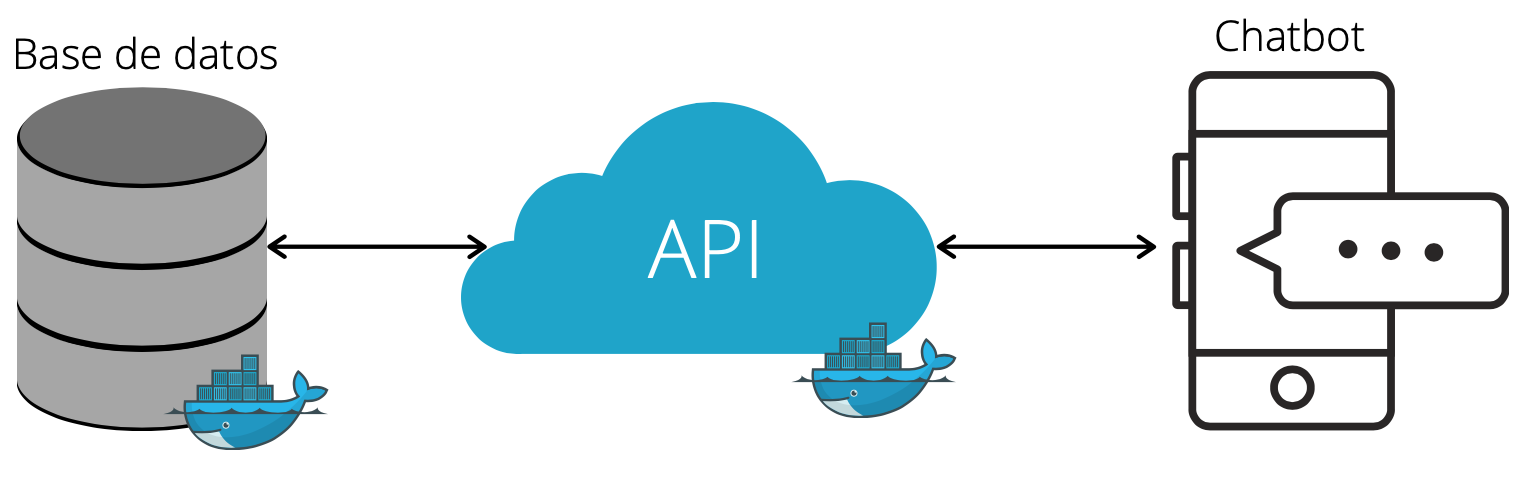
\includegraphics[scale=0.4]{{include/figuras/ArquitecturaGeneral.png}}
    \caption{Arquitectura general}
    \label{fig:arquitectura_general}
\end{figure}

Como se puede observar en la figura \ref{fig:arquitectura_general}, la API RestFul es el software encargado de gestionar e interactuar con la base de datos, sirviendo los datos a los usuarios. Para que el proyecto sea lo más escalable posible se ha decidido separar los servicios de forma que estén débilmente acopladas. 

\section{Herramientas utilizadas}

\subsection{Base de Datos}
Para el proyecto Sonidos del Cielo hemos elegido MongoDB. En gran parte debido a que es una herramienta perfecta para entornos con bajos recursos de computación, no es necesario pagar ningún tipo de licencia, posee una gran comunidad y muy buena documentación, además de muy escalable. La ventaja principal de MongoDB es que los documentos no tienen que seguir una estructura definida, es decir, se puede trabajar con documentos independientes, modificar el contenido de uno de forma individual y no afectar a la estructura.

\begin{figure}[h]
    \centering
    
\includegraphics[scale=0.2]{include/figuras/mongo.png}
    \caption{Logo de MongoDB}
    \label{fig:mongo}
\end{figure}

La característica principal de MongoDB es la velocidad, dado que está escrito en C++ tiene la capacidad de aprovechar los recursos del sistema de una manera eficiente, es decir, tiene un gran balance entre funcionalidad y rendimiento gracias a su sistema de consulta de contenidos. Las características principales de la plataforma son:

\begin{itemize}
    \item Consultas ad-hoc: se pueden realizar todo tipo de consultas. Podemos buscar por campos como si de una base de datos relacional se tratase pero además podemos buscar por rango, mediante expresiones regulares.
    \item Indexación: el concepto es muy parecido al utilizado en las bases de datos relacionales, sin embargo, en MongoDB se puede indexar cualquier campo documentado e incluir múltiples índices secundarios.
    \item Balanceo de carga: MongoDB posee la capacidad de ejecutarse de manera simultánea en múltiples servidores, dando un servicio de balanceo de carga o de replicación de datos, de manera que es posible mantener el funcionamiento del sistema en caso de un fallo de hardware.
    \item Almacenamiento de archivos: puede ser utilizado también como almacenamiento de archivos, esta función, conocida como GridFS está incluida en la distribución oficial y permite manipular archivos y su contenido.
    \item Ejecución de JavaScript en el lado del servidor: es posible realizar consultas utilizando código escrito en JavaScript, haciendo que estas sean enviadas directamente a la base de datos para ser ejecutadas.
\end{itemize}

\subsubsection{Funcionamiento de MongoDB}
MongoDB está orientado a documentos. Esto significa que en lugar de guardar los datos en registros se guardan en documentos BSON, que no es otra cosa que un fichero JSON binario.
Esto es una de las grandes diferencias respecto a las bases de datos relacionales. 
MongoDb se compone de colecciones que a su vez está formado por documentos documentos. 

Si hiciésemos una comparación con los elementos de una base de datos relacional, se trataría de una tabla. Dentro de cada colección existen múltiples documentos que están compuestos de pares Clave-Valor. 
La principal diferencia respecto a una base de datos relacional es que no es necesario que los documentos de una misma colección tengan el mismo formato ni los mismos campos.

\subsubsection{Arquitectura de la Base de Datos}

Las tablas obtenemos desde ficheros que se encuentran en un servidor del Spanish Virual Observatory (SVO) dentro del Departamento de Arquitectura y Tecnología de Sistemas Informáticos de la Escuela Técnica Superior de Ingenieros Informáticos de la Universidad Politécnica de Madrid. A partir de este fichero se crean las tablas que se aprecian en la figura \ref{fig:tablas_base_datos}

\begin{figure}[H]
    \centering
    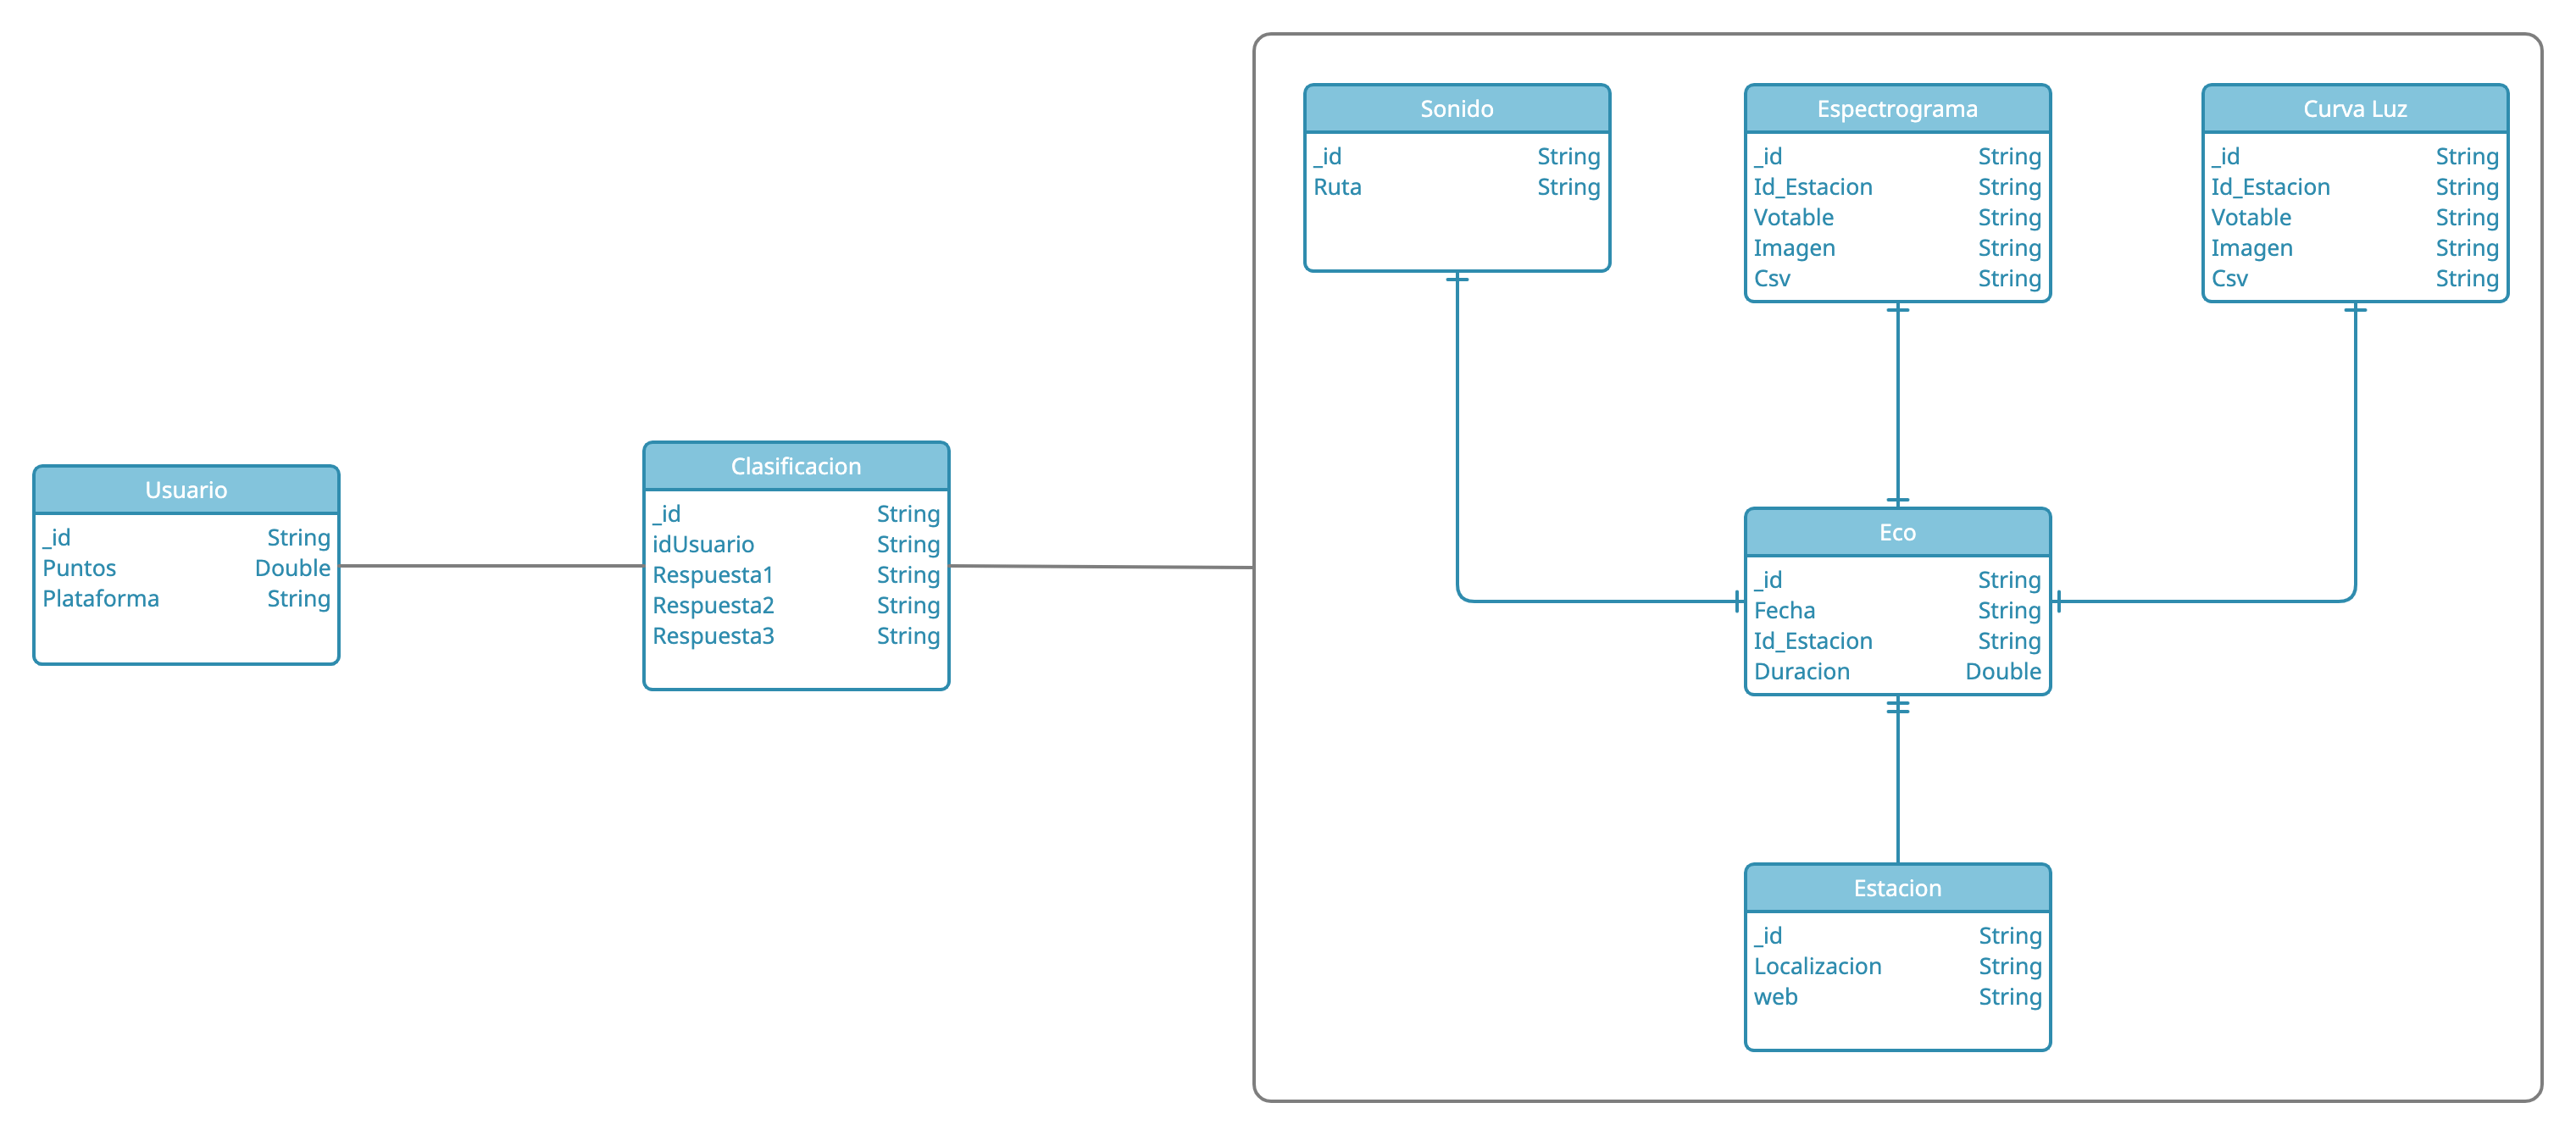
\includegraphics[width=\textwidth]{include/figuras/Tablas.png}
    \caption{Colecciones de la base de datos}
    \label{fig:tablas_base_datos}
\end{figure}

Aunque hemos explicado anteriormente que no es estrictamente necesario que existan relaciones entre las tablas, en este proyecto si que es necesario puesto que varias tablas proceden del mismo meteoroide.

Una vez creada la base de datos y establecer usuarios para restringir el acceso a la misma, podemos realizar operaciones de consulta, inserción, eliminación y actualización de documentos, colecciones y bases de datos a través de la consola incluida dentro del paquete de instalación de MongoDB. 

\begin{figure}[H]
    \centering
    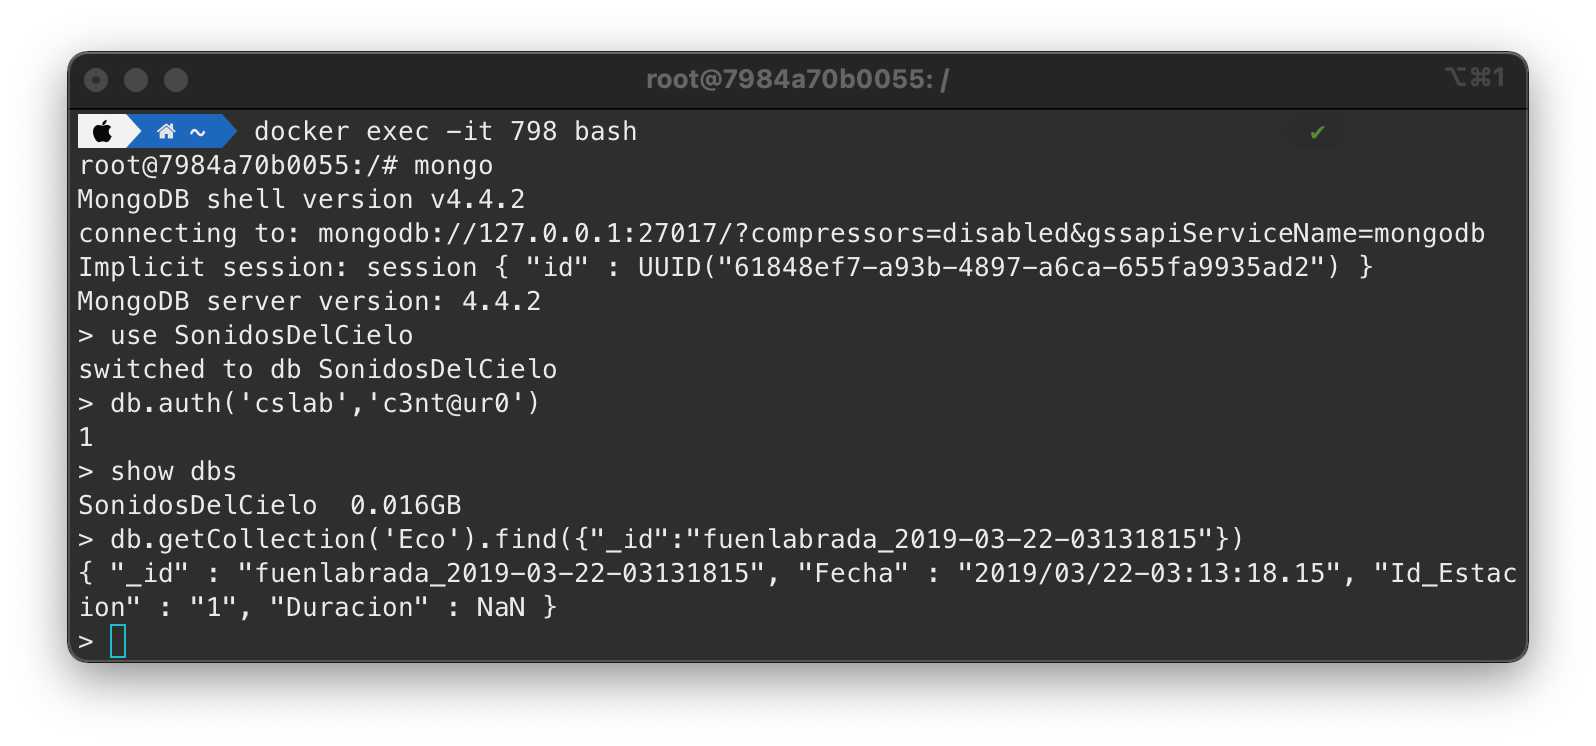
\includegraphics[scale=0.4]{include/capturas/TerminalMongo.png}
    \caption{Operación con terminal de mongo}
    \label{fig:terminal_mongo}
\end{figure}

También existen herramientas gráficas para modificar cualquier parámetro de una base de datos en Mongo como puede ser MongoDB Compass o Robo 3T. Estas herramientas proporcionan una vía más sencilla y visual para trabajar con las bases de datos además de no tener que aprender o buscar dentro de la documentación los comandos necesarios para manejar una interfaz de línea de comandos propietaria. Aunque también nos permite el ejecutar comandos como si se tratase del terminal como se puede observar en la figura \ref{fig:robo3t}.

\begin{figure}[H]
    \centering
    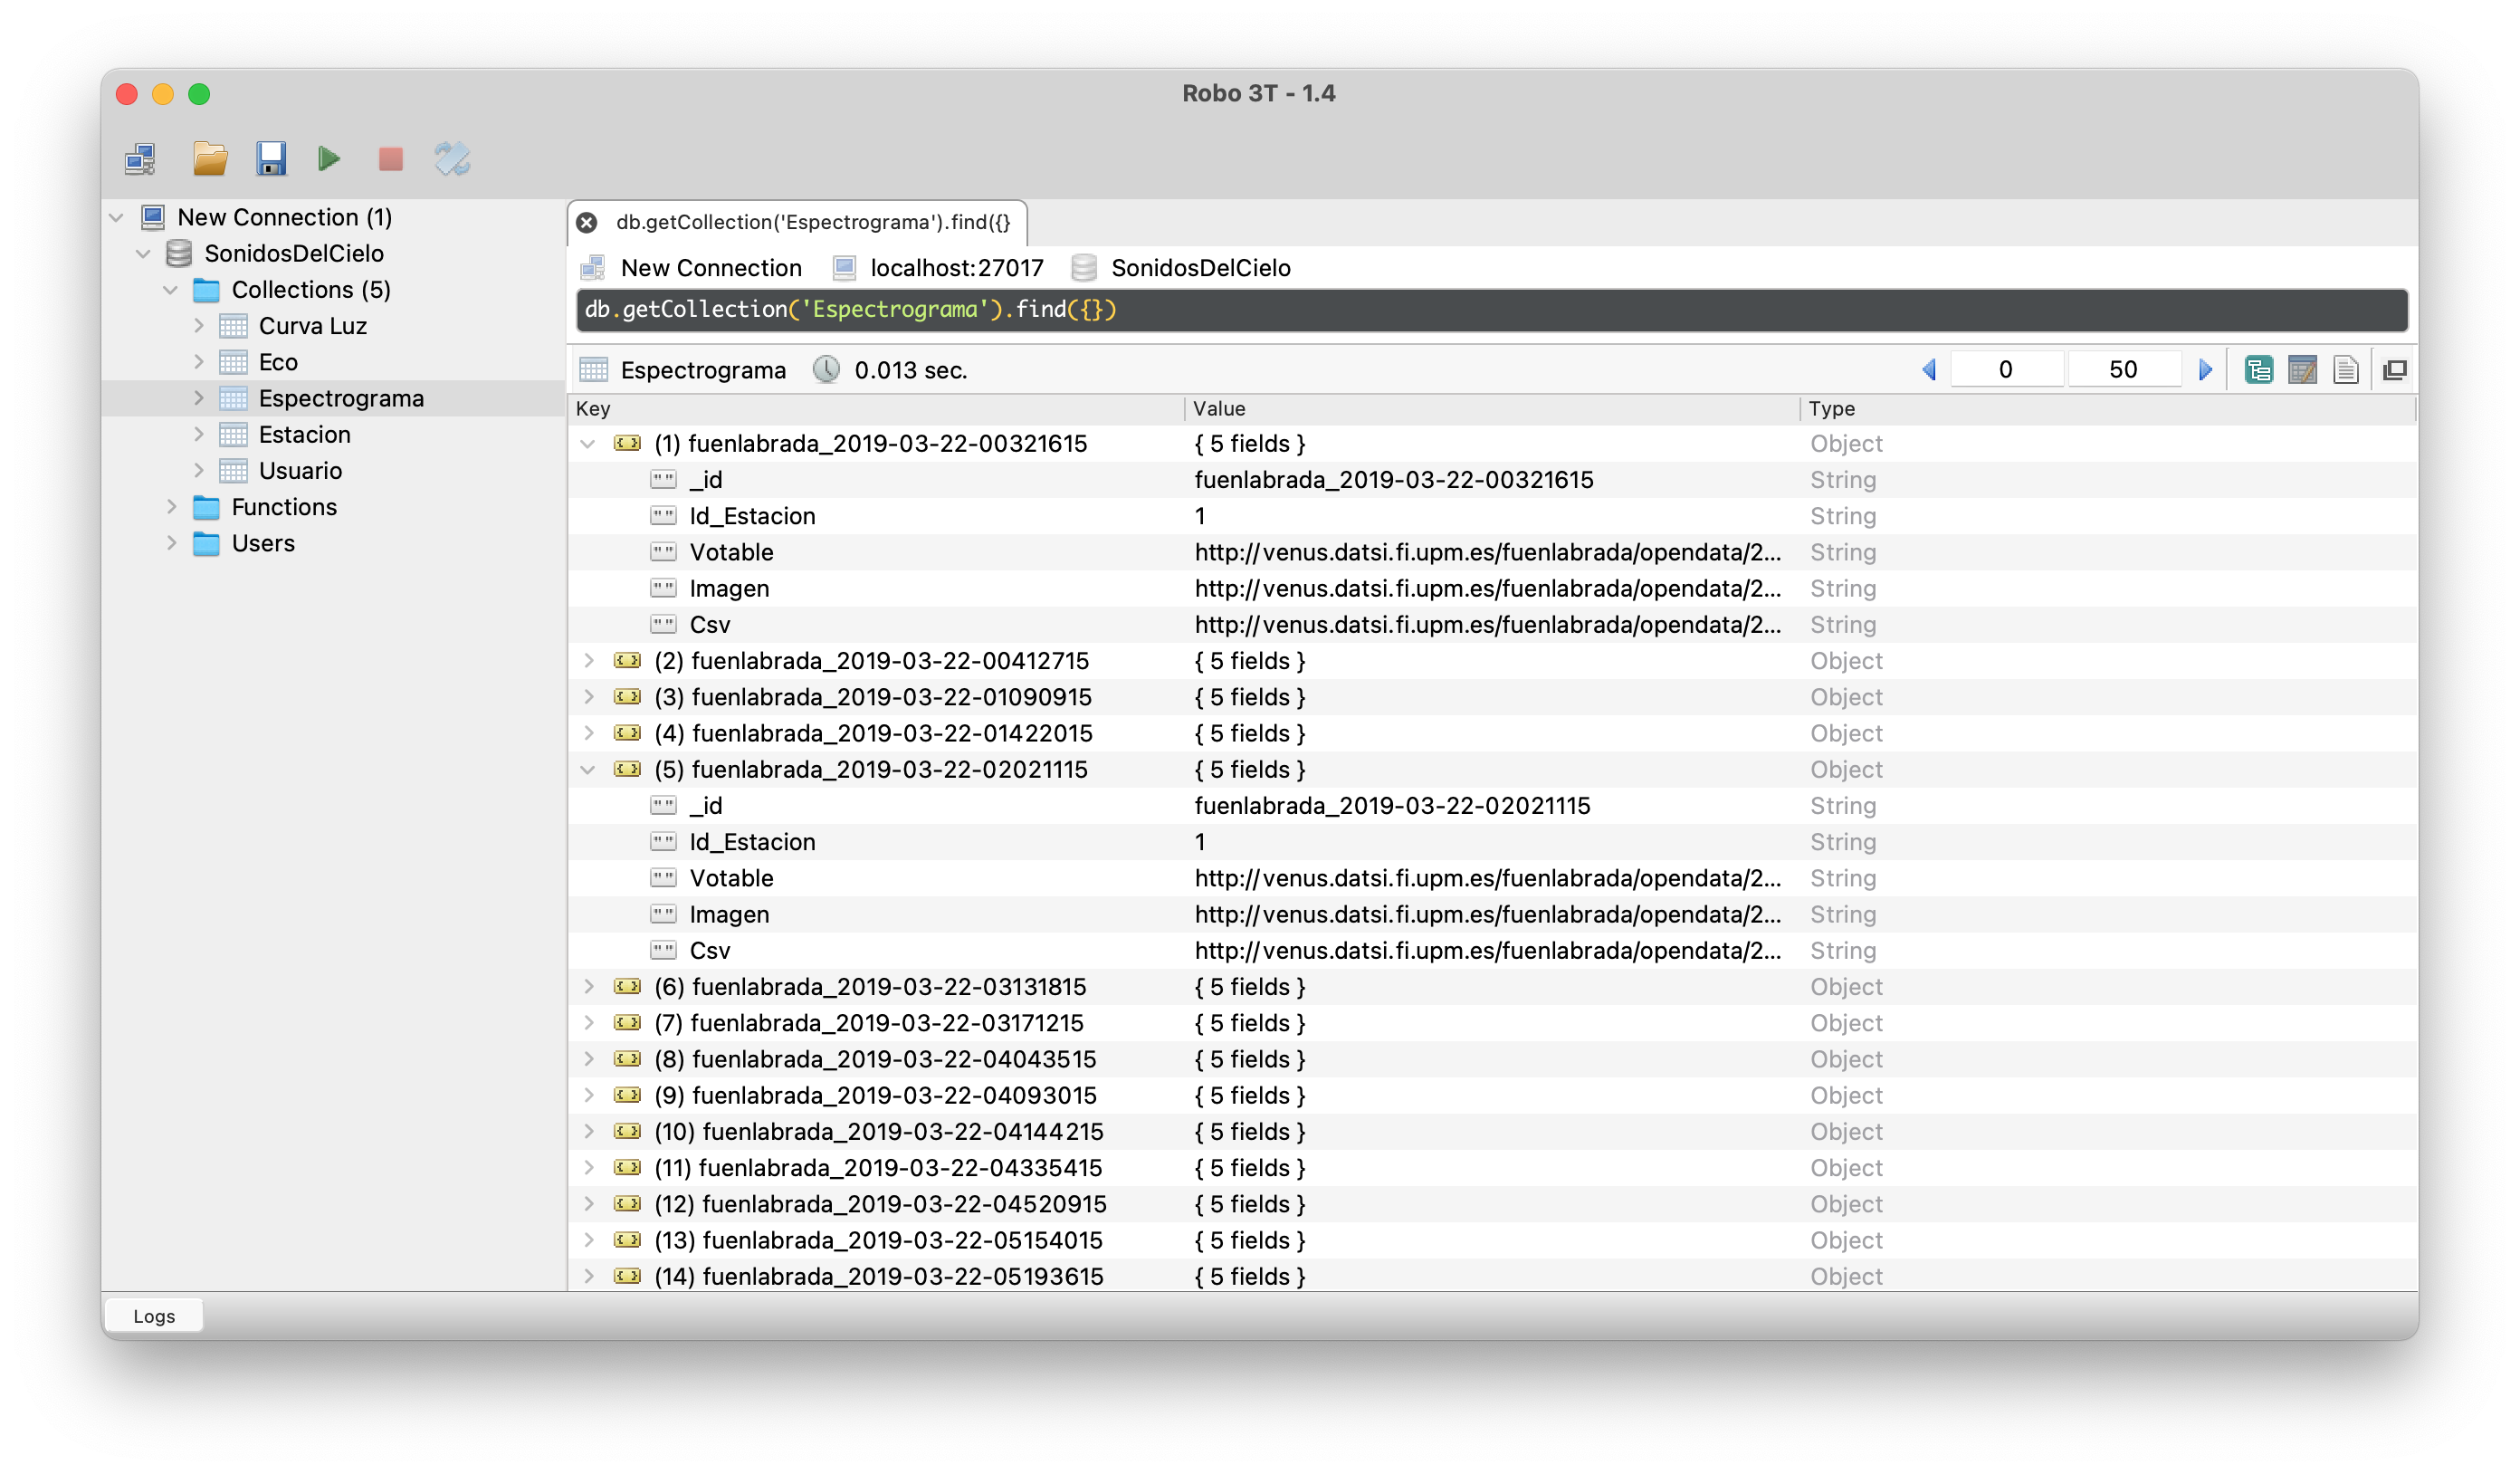
\includegraphics[scale=0.3]{include/capturas/Robo3T.png}
    \caption{Interfaz de Robo3T}
    \label{fig:robo3t}
\end{figure}

\newpage
\subsection{Lenguaje de Programación Python}

Tanto para la carga de los documentos en la base de datos como para el desarrollo del chatbot ha sido necesario el uso del lenguaje de programación Python. Python es un lenguaje de programación creado a finales de los años 80 por Guido van Rossum en el Centro para las Matemáticas y la Informática de Países Bajos. Este lenguaje posee una gran flexibilidad que produce código ordenado, limpio y fácilmente legible. Sus principales características pueden resumirse en las siguientes\cite{python}:

\begin{figure}[h]
    \centering
    
\includegraphics[scale=0.4]{include/figuras/python.png}
    \caption{Logo de Python}
    \label{fig:Python}
\end{figure}

\begin{itemize}
    \item Gratis: No es necesario pagar licencia para utilizarlo
    \item Interpretado: se ejecuta sin tener que pasar por un compilador y los errores son detectados en tiempo de ejecución.
    \item Multiplataforma: está disponible para Windows, Mac y Linux. 
    \item Tipado dinámico: las variables declaradas se comprueban durante el tiempo de ejecución.
    \item Multiparadigma: soporta programación funcional, programación imperativa, declarativo, modular, dirigido a eventos, programación asíncrona, lógico, estructurado, con restricciones y programación orientada a objetos.
\end{itemize}

Es un lenguaje que se tiene una curva de aprendizaje muy rápida, además cuenta con una gran comunidad lo que hace que existan librerías y módulos especializados desarrollados como \textit{pandas} (tratamiento de datos) \textit{librosa} (para procesamiento de audio), \textit{sklearn} (machine-learning) o frameworks como \textit{Django} (para desarrollo web) o en nuestro caso, \textbf{RASA} para desarrollar un chatbot. 

\subsection{Arquitectura aplicación RestFul}

La aplicación RestFul no es más que el software que hace de intermediario para enviar información de la base de datos al cliente o para insertar datos desde el cliente a la base de datos \cite{apiRest}. El cliente es aquel que consume la información, en nuestro caso, el chatbot. El servidor se ha desarrollado en Node.js. Fue diseñado para la construcción de aplicaciones escalables, siendo un punto muy a favor para nuestra elección. 

\begin{figure}[h]
    \centering
    
\includegraphics[scale=0.15]{include/figuras/node.jpg}
    \caption{Logo de Node.js}
    \label{fig:node}
\end{figure}

\subsubsection{Funcionamiento de Node.js}

Node.js es un entorno de ejecución de JavaScript \cite{javascript} orientado a eventos asíncronos. Comparándolo con servicios web clásicos donde cada nueva conexión genera un nuevo subproceso (ocupando memoria RAM del sistema) y normalmente ocupando toda la memoria RAM disponible. Node.js trabaja en un subproceso únicamente, utilizando el modelo entrada y entrada sin bloqueo de la salida, esto permite soportar una cantidad enorme de conexiones simultáneas mantenidas dentro del bucle de eventos. El servidor consta de un subproceso que trata un evento tras otro.
Cuando se produce una nueva solicitud se genera un evento. El servidor comienza a procesarlo y cuando se produce una operación de bloqueo de la entrada/salida, no espera a que se termine sino que se crea una \textit{función de callback}. El servidor comienza instantáneamente a procesar otro evento y cuando termine la operación de entrada/salida, seguirá trabajando en la solicitud ejecutando la función de callback tan pronto como sea posible.

Gracias a este mecanismo, el servidor no necesita crear subprocesos lo que significa que no tiene apenas sobrecarga. Además, puesto que queremos tratar las peticiones de los usuarios, la mejor manera de hacerlo es de forma asíncrona así no es necesario esperar a que se traten las peticiones realizadas con anterioridad.


\subsubsection{Ventajas de utilizar Node.js}

Node.js es la plataforma de software más utilizada en la actualidad por encima de otros entornos de ejecución y lenguajes de programación como pueden ser C o PHP a la vez que tiene un tiempo de ejecución mucho mayor. No es un lenguaje de programación complejo pero requiere una mayor comprensión y cantidad de líneas de código que PHP. Cuando hablamos de Node.js hay algo que es necesario destacar, el conocido como Node Package Manager (NPM) que viene por defecto con la instalación de Node.js.


\subsubsection{Librerías utilizadas}A continuación se especificarán los paquetes utilizados para el desarrollo de la API RestFul.

\begin{itemize}
    \item Async: es un módulo que proporciona funciones sencillas para el tratamiento de llamadas asíncronas.
    \item Body-parser: es un middleware encargado de extraer todo el cuerpo de una request entrante y la muestra en el \textit{req.body} 
    \item Cors: este paquete se encarga de controlar el mecanismo que utilizan las cabeceras HTTP para permitir que un \textit{user agent} tenga permiso para acceder a ciertos recursos desde un servidor en un dominio distinto al que pertenece.
    \item Dotenv: Sirve para cargar variables de entorno desde un fichero .env.
    \item Express: es un framework de desarrollo web inspirado en Sinatra y por consiguiente, el estandar de la gran mayoría de aplicaciones de Node.js. Es la librería que utilizaremos para desplegar el servidor de la API.  
    \item Mongoose: es una herramienta encargada del tratamiento de bases de datos MongoDB de manera asíncrona.
    \item Nodemon: este paquete simplifica la tarea de volver a iniciar la aplicación cada vez que se realice un cambio en el código. Es un demonio que se ejecuta en segundo plano y es el encargado de comprobar los cambios e iniciar el servidor.
    \item Swagger-Jsdoc: genera definiciones OpenAPI a partir de comentarios JSDoc.
    \item Swagger-UI-Express: crea la interfaz de usuario de Swagger en base a las definiciones creadas con Swagger-JSDoc.
\end{itemize}

\subsection{Visual Studio Code}

Visual Studio Code es un editor gratuito y de código abierto desarrollado por Microsoft y que se distribuye mediante licencia MIT. \footnote{Licencia MIT: licencia creada en el Instituto Tecnológico de Massachusetts, se trata de una licencia de software libre que impone muy pocas restricciones en su reutilización} Se trata de un software multiplataforma (Windows, macOS y Linux).
Está creado en NodeJS y Electron \cite{electron} y con Blink como motor gráfico.

Se trata de un editor hackeable, es decir, permite modificar el comportamiento del editor completamente (tema del editor, atajos de teclado, preferencias, etc), tiene soporte para Git integrado, autocompletado de código, terminal integrado y debugger.

Además posee una biblioteca de extensiones \ref{fig:vscode} mediante la cual puedes añadir herramientas que ayuden en los proyectos o visualizar el código de forma más eficiente. También posees un live server a través del cual puedes visualizar código web en tu navegador predeterminado inmediatamente según guardas el código sin ser necesario refrescar.

\begin{figure}[h]
    \centering
    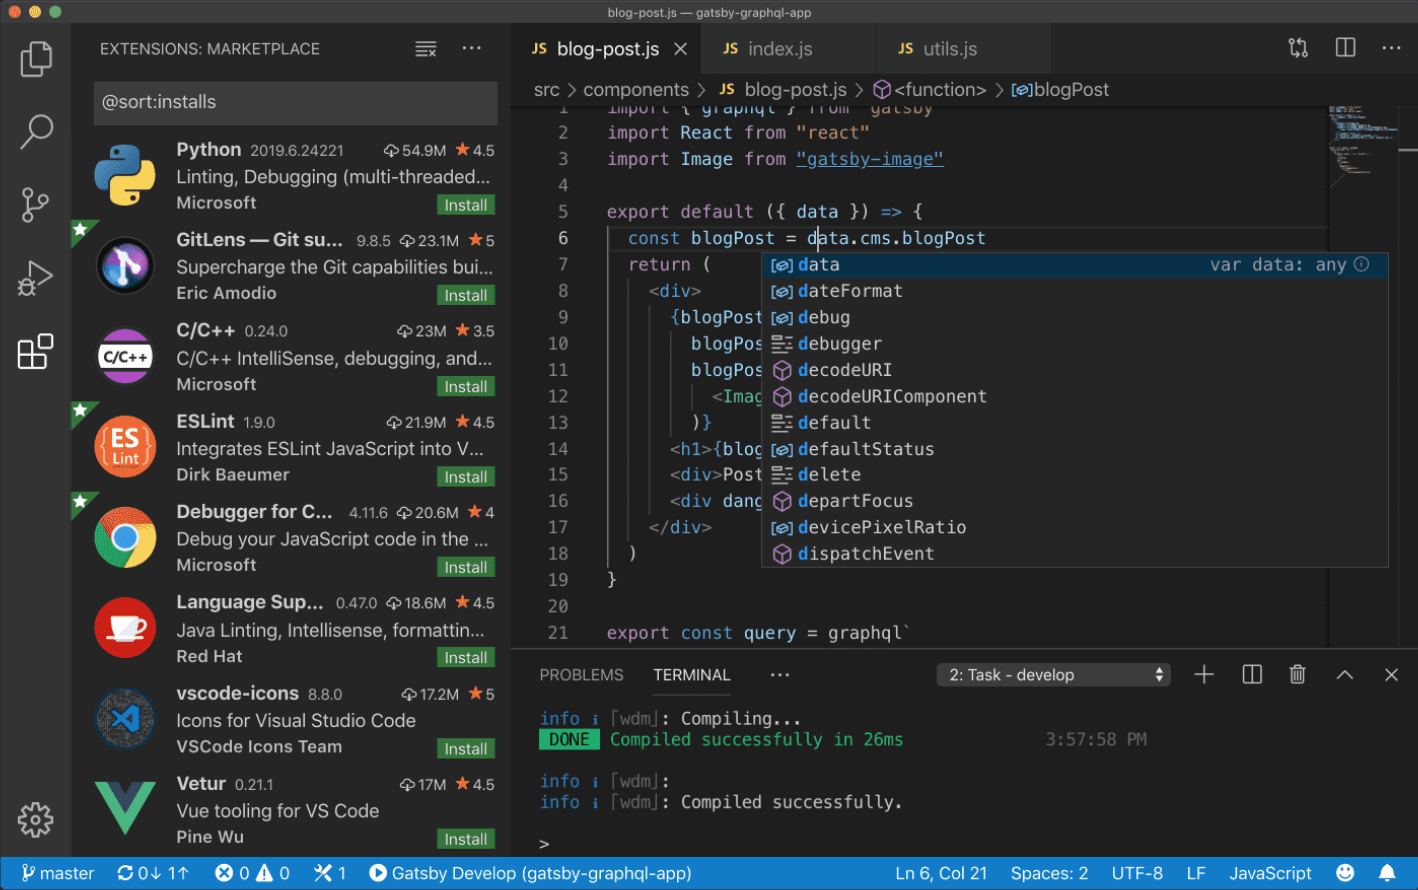
\includegraphics[width=\textwidth]{include/figuras/VSCode.png}
    \caption{Visual Studio Code}
    \label{fig:vscode}
\end{figure}

A continuación se explicará brevemente las extensiones utilizadas:.

\begin{itemize}
    \item \textbf{Docker}: esta extensión simplifica la forma en la que construir, controlar y desplegar aplicaciones \textit{dockerizadas}, además proporciona herramientas dentro de un contenedor para realizar debugging de aplicaciones desarrolladas en Node.js, Python y .NET Core.
    \item \textbf{YAML}: proporciona compatibilidad completa con el lenguaje YAML con compatibilidad para la sintaxis de Kubernetes.
    \item \textbf{MarkdownLint}: incluye una biblioteca de reglas para entender los estándares y la coherencia de los archivos Markdown. 
    \item \textbf{TODO Tree}: esta extensión busca rápidamente las etiquetas TODO y FIXME y las muestra en un árbol. 
\end{itemize}


\subsection{Git y Github}


En el desarrollo de cualquier proyecto de software surge la necesidad de gestionar los cambios que se producen entre versiones diferentes de un mismo código fuente. Habitualmente este proceso se inicia utilizando sufijos en los ficheros que se modifican (v1, antiguo, nuevo) pero este proceso no es ni eficiente ni práctico, mucho menos si trabajamos en equipo, dando lugar a la eliminación de archivos válidos realizados por otros componentes del equipo, incapacidad de conocer que cambios se han realizado, etc.

En todo proyecto, más tarde o más temprano aparece la necesidad de trabajar en distintas ramas, en el entorno empresarial suelen ser desarrollo y producción. En la rama de desarrollo se procede a introducir las nuevas modificaciones y en la rama de desarrollo las versiones estables del programa.

Para ayudarnos con esta tarea aparecen soluciones como Git, CVS que realizan tareas fundamentales como pueden ser:

\begin{figure}[h]
    \centering
    
\includegraphics[scale=0.1]{include/figuras/Git.png}
    \caption{Logo de Git}
    \label{fig:git}
\end{figure}

\begin{itemize}
    \item Comparación de ficheros de tal manera que rápidamente encontremos las diferencias entre los dos. 
    \item Restauración de versiones anteriores.
    \item Fusionar versiones.
    \item Trabajar con varias ramas de un proyecto.
    \item Facilitar la colaboración.
\end{itemize}


En el caso del proyecto Sonidos del Cielo la herramienta de control de versiones utilizada ha sido \textbf{Git}. 

Git surgió de la mano de Linus Torvals \cite{torvalds2005git}, es un sistema de control de versiones de código abierto, multiplataforma, lo que nos permite crear repositorios en cualquier sistema operativo. Existen gran variedad de herramientas gráficas para manejar Git pero lo más utilizado el la línea de comandos dado que, una vez aprendidos los comandos básicos, nos permite realizar las operaciones con mayor velocidad. 

Github es un servicio para alojar repositorios creado en San Francisco en el año 2008. Está pensado para compartir código fuente en cualquier lenguaje de programación y dejarlo a disposición de cualquiera que quiera reutilizarlo siempre y cuando haya permiso para ello. Si cualquier otro usuario que no sea el creador del proyecto puede realizar un \textit{fork}, un fork no es otra cosa sino que la creación de una copia de otro proyecto en otro repositorio.
También hay repositorios privados en los que sólo el creador del repositorio y las personas a las que el de acceso podrán participar.

\begin{figure}[h]
    \centering
    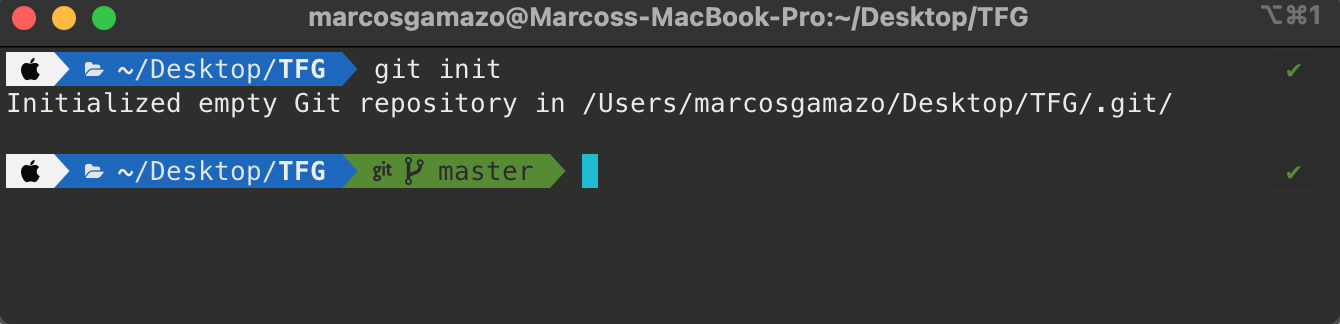
\includegraphics[width=\textwidth]{include/capturas/gitInit.png}
    \caption{Inicialización de repositorio en Git}
    \label{fig:git_init}
\end{figure}


Github cuenta con diversas herramientas de las que las más destacables son:

\begin{itemize}
    \item Gollum: permite la creación de wikis basadas en git.
    \item Sistema de revisión de código: para añadir comentarios y discutir sobre las modificaciones realizadas.
    \item Visor de ramas: dónde podremos revisar los avances del repositorio.
    \item Herramienta de seguimiento de problemas: nos permite abrir tickets de incidencias o mejoras a realizar.
\end{itemize}


\subsection{Swagger}
Una de las partes más importantes en cualquier proyecto es la documentación del código. Es muy habitual en nuestro campo que hay que modificar, mantener o simplemente que utilizar código desarrollado por otra persona y se convierte en una tarea ardua que obliga a invertir demasiado tiempo en comprenderlo. 

Para evitar estas situaciones es habitual adaptar herramientas que permitan comentar el código fuente del software que desarrollemos de tal manera que sea legible por cualquier persona. En el proyecto Sonidos del Cielo se ha decidido seleccionar la herramienta \textit{Swagger}\cite{Swagger} para documentar la API RestFul. 

Swagger se compone de una serie de herramientas, reglas y especificaciones mediante las cuales podremos documentar y probar una API de una manera sencilla. La principal baza para utilizar Swagger es que es realmente sencilla de implementar y cualquier persona es capaz de entenderlo, tenga conocimientos de programación o no. Esto es posible gracias a \textbf{Swagger UI}, es una de las características más importantes de la plataforma, esta herramienta nos permite organizar las operaciones CRUD de la API basándose en los ficheros YAML o JSON y creando un entorno interactivo.

\begin{figure}[H]
    \centering
    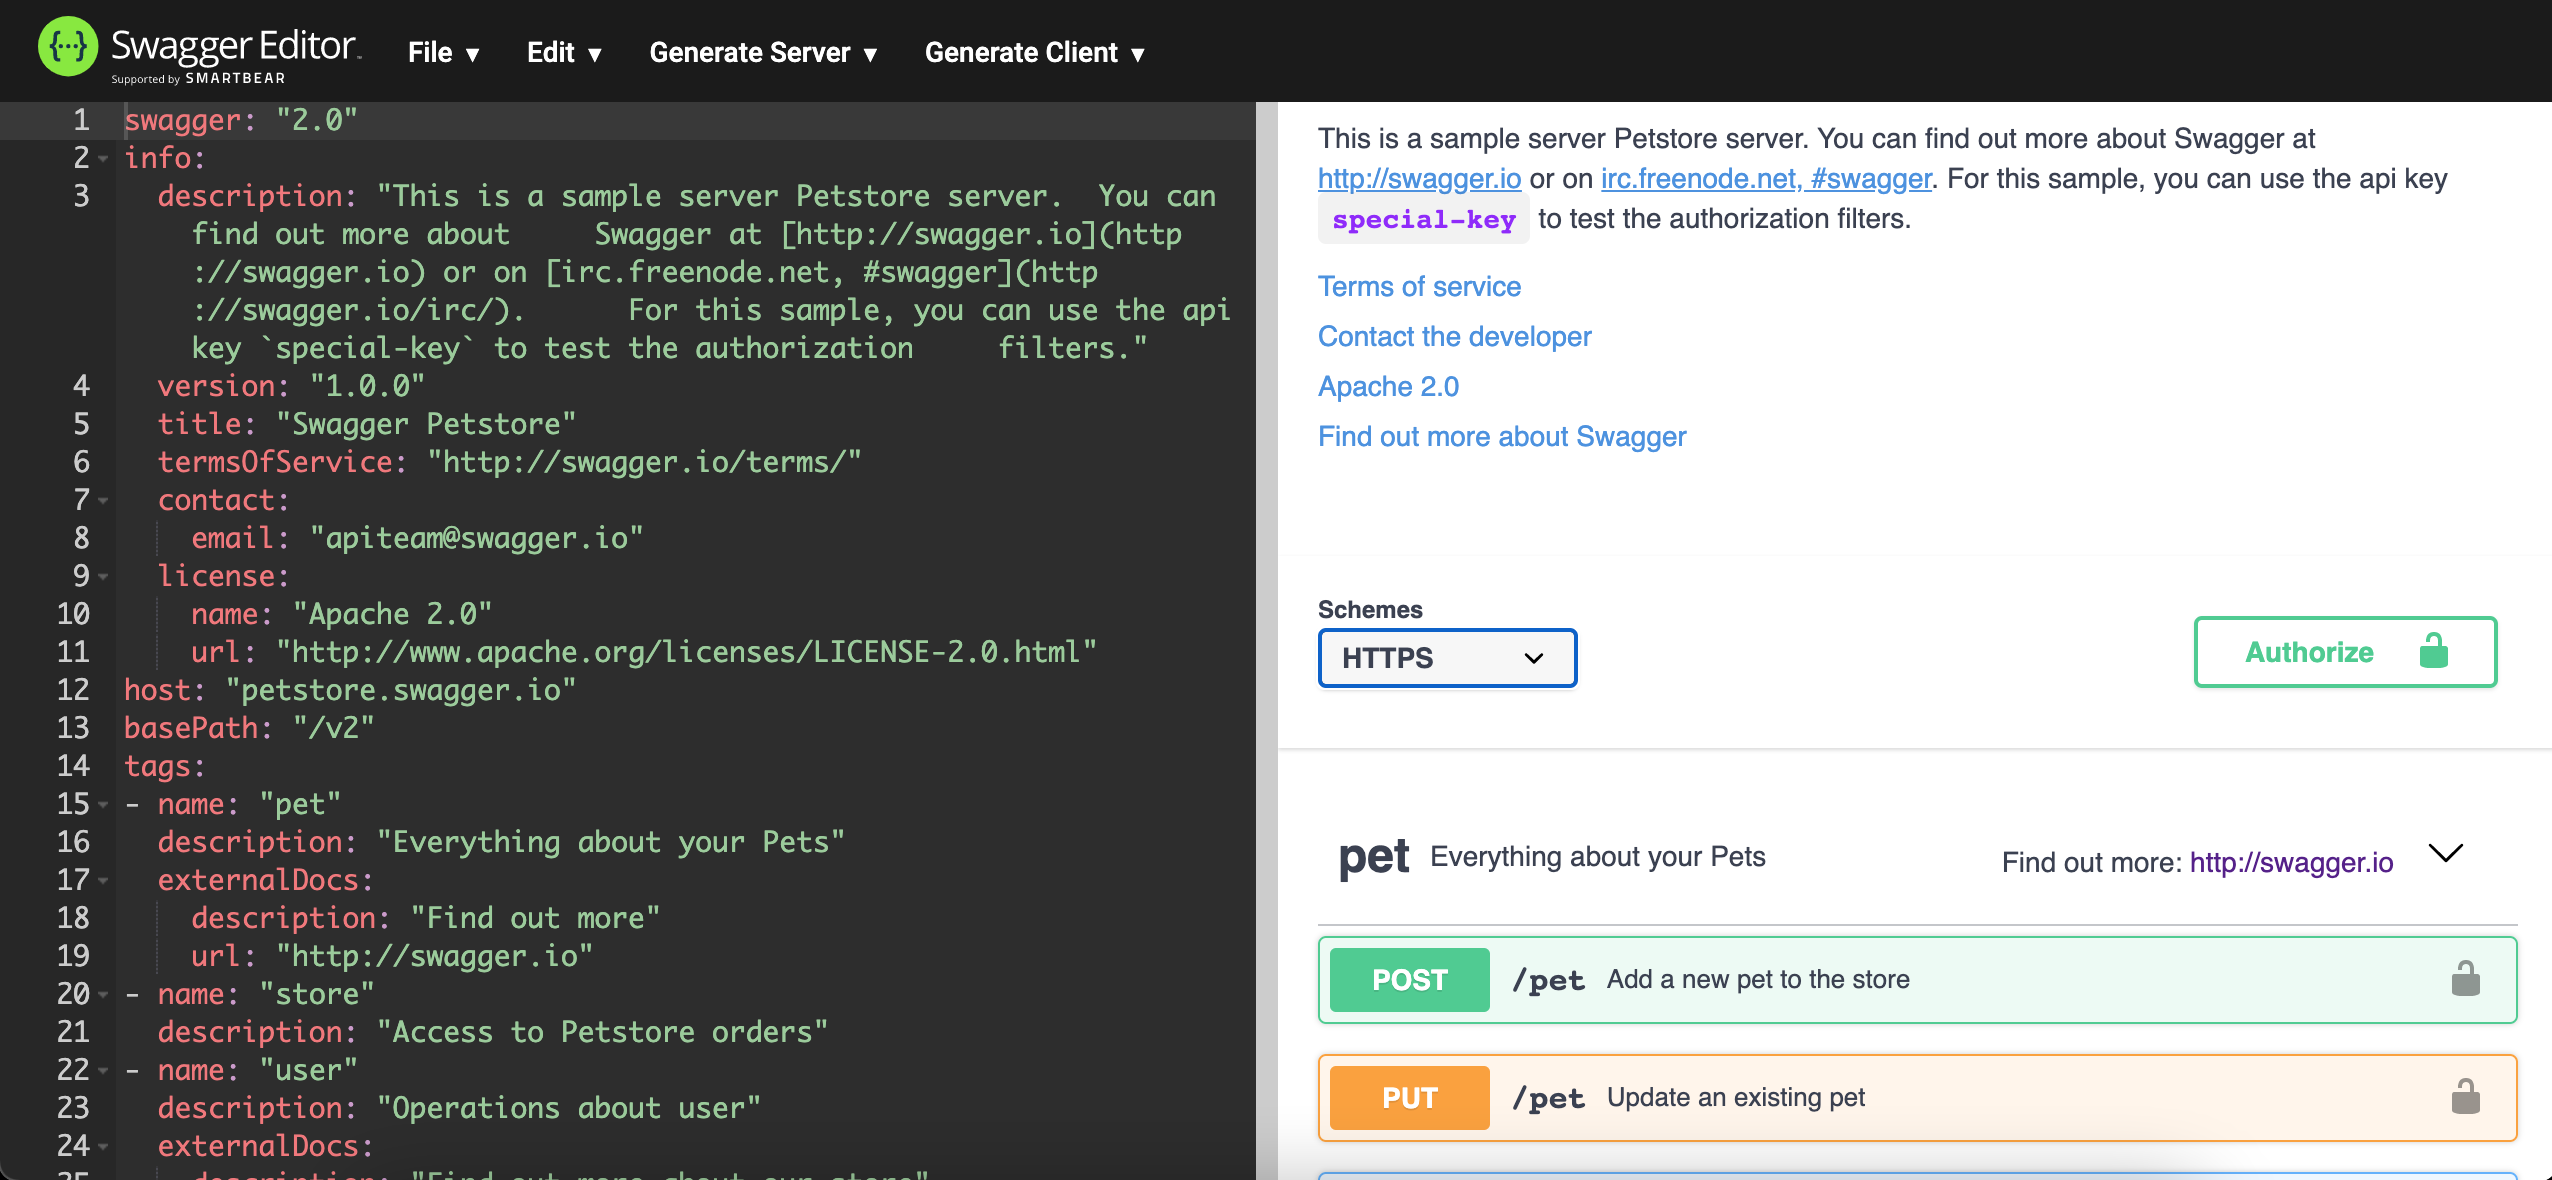
\includegraphics[width=\textwidth]{include/capturas/SwaggerEditorOnline.png}
    \caption{Swagger Editor}
    \label{fig:swagger_online}
\end{figure}

Para esta tarea podemos utilizar la versión del editor en línea, \textit{Swagger editor} que proporciona la plataforma como se muestra en la figura \ref{fig:swagger_online}, esta herramienta nos indicará los errores que se hayan cometido y además brindará sugerencias y alternativas para mejorar la documentación.

Nuestra implementación pasa por la utilización de Swagger y Swagger UI como varios paquetes instalables dentro de Node.js \cite{DocumentWithSwagger} a través del instalador npm. Dentro de la definición del servidor se incluyen las opciones del servidor como se muestra en la figura \ref{fig:swagger_options} entre las que cabe destacar la versión del API Rest, la versión OpenAPI o la información del proyecto.

\begin{figure}[H]
    \centering
    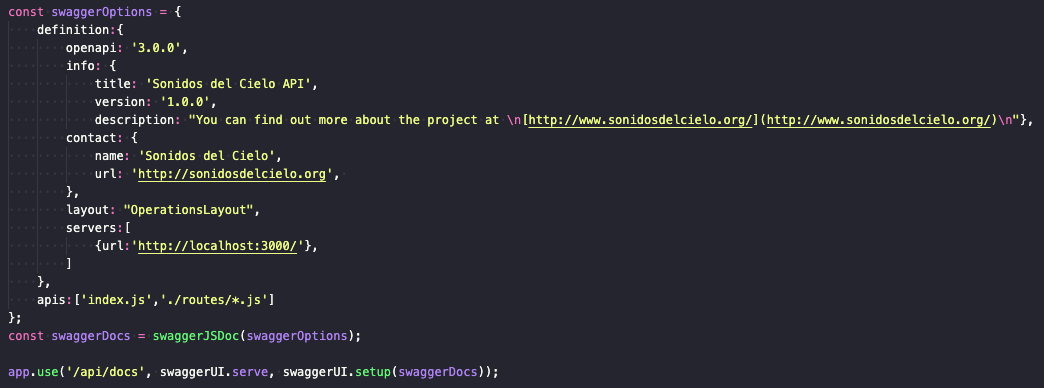
\includegraphics[width=\textwidth]{include/capturas/SwaggerOptions.png}
    \caption{Opciones del servidor de Swagger}
    \label{fig:swagger_options}
\end{figure}

Una vez establecido los parámetros básicos del servidor y haber definido los componentes que forman la API Rest es momento de añadir el código YAML \cite{AutomaticAPIDocumentation} para crear la documentación de los distintos métodos. En ese código se indica el tipo de formato que se produce, \textbf{JSON} en nuestro caso, los códigos de respuesta que proporciona la API.

\begin{figure}[h]
    \centering
    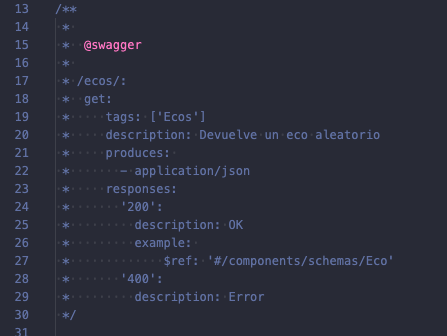
\includegraphics[scale=0.7]{include/capturas/SwaggerYAML.png}
    \caption{Definición Swagger}
    \label{fig:swagger_definition}
\end{figure}

Una vez estén comentados todos los métodos de nuestra API en los distintos \textit{endpoints} que se hayan definido se mostrará una interfaz gráfica una vez accedamos a la url indicada en las opciones que se observan en la figura \ref{fig:swagger_options} dando como resultado la interfaz que se observa en la figura \ref{fig:swagger_ui}

\begin{figure}[H]
    \centering
    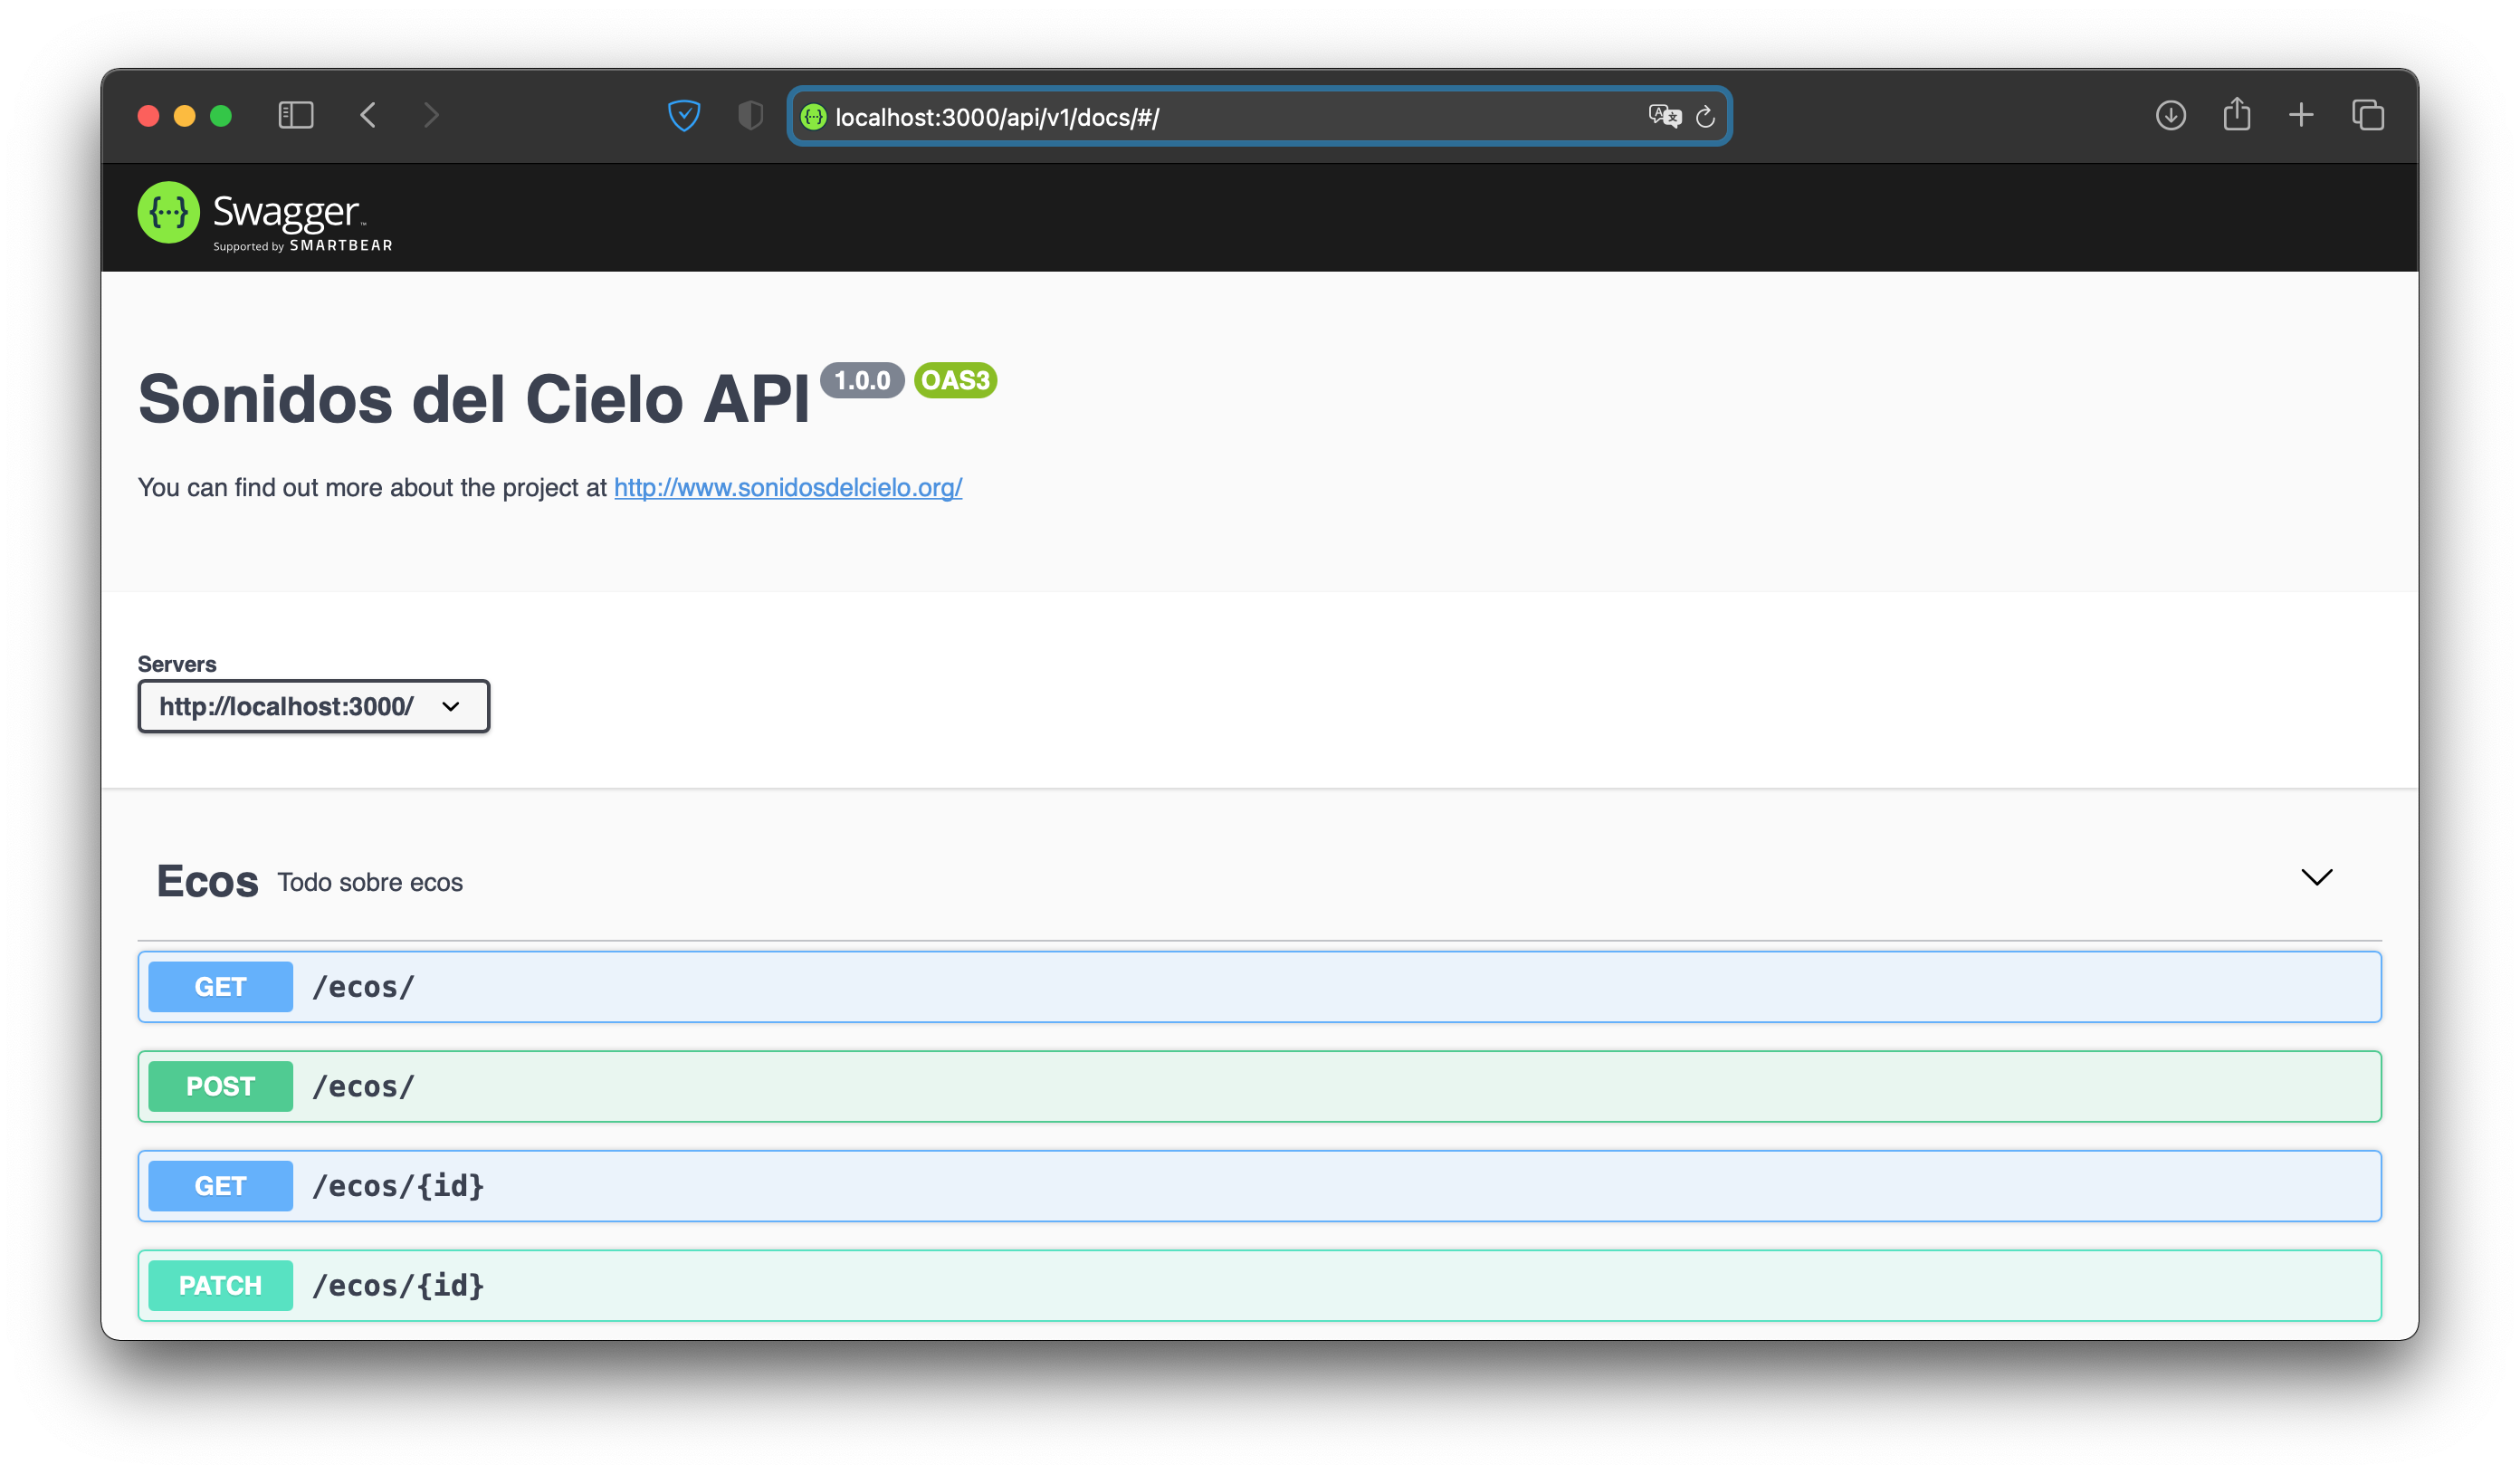
\includegraphics[width=\textwidth]{include/capturas/SwaggerUI.png}
    \caption{Interfaz web Swagger}
    \label{fig:swagger_ui}
\end{figure}

\subsection{Postman}
Durante el desarrollo del servicio de la API Rest es necesario comprobar si las operaciones se están realizando correctamente y si se arrojan los resultados esperados. Para comprobarlo existen herramientas diversas que van desde una sentencia \textit{curl} desde cualquier terminal de un sistema operativo a la utilización de herramientas gráficas que nos proporcionen información extra sobre las explotación de los métodos creados y sus resultados. 

En esta última dirección, se hallan varias herramientas como pueden ser Advanced REST Client, Insomnia Rest Client, soapUI, Postman, etc. Para este trabajo se ha seleccionado \textbf{Postman} por el hecho de conocer la herramienta y su funcionamiento con anterioridad.

En el momento de su creación, Postman fue diseñado como una extensión del navegador Google Chrome aunque en la actualidad ya existen aplicaciones nativas para Windows, Linux y macOS. Agrupa una variedad de utilidades y herramientas que ayudan en el diseño y desarrollo de un API Rest. Algunas de las más destacables son:

\begin{itemize}
    \item Creación de peticiones a APIs
    \item Desarrollo de test de validación de la API
    \item Entornos de trabajo
\end{itemize}

El interés principal de la utilización de esta herramienta es para realizar peticiones a la API y tener la capacidad de generar colecciones de peticiones que nos permitan testear de una forma sencilla y rápida.
Todas las llamadas que se realicen en la API se guardan en colecciones. Todas las llamadas guardadas se pueden exportar a varios lenguajes de programación como se ve en la siguiente figura \ref{fig:postman_snippet}.

\begin{figure}[H]
    \centering
    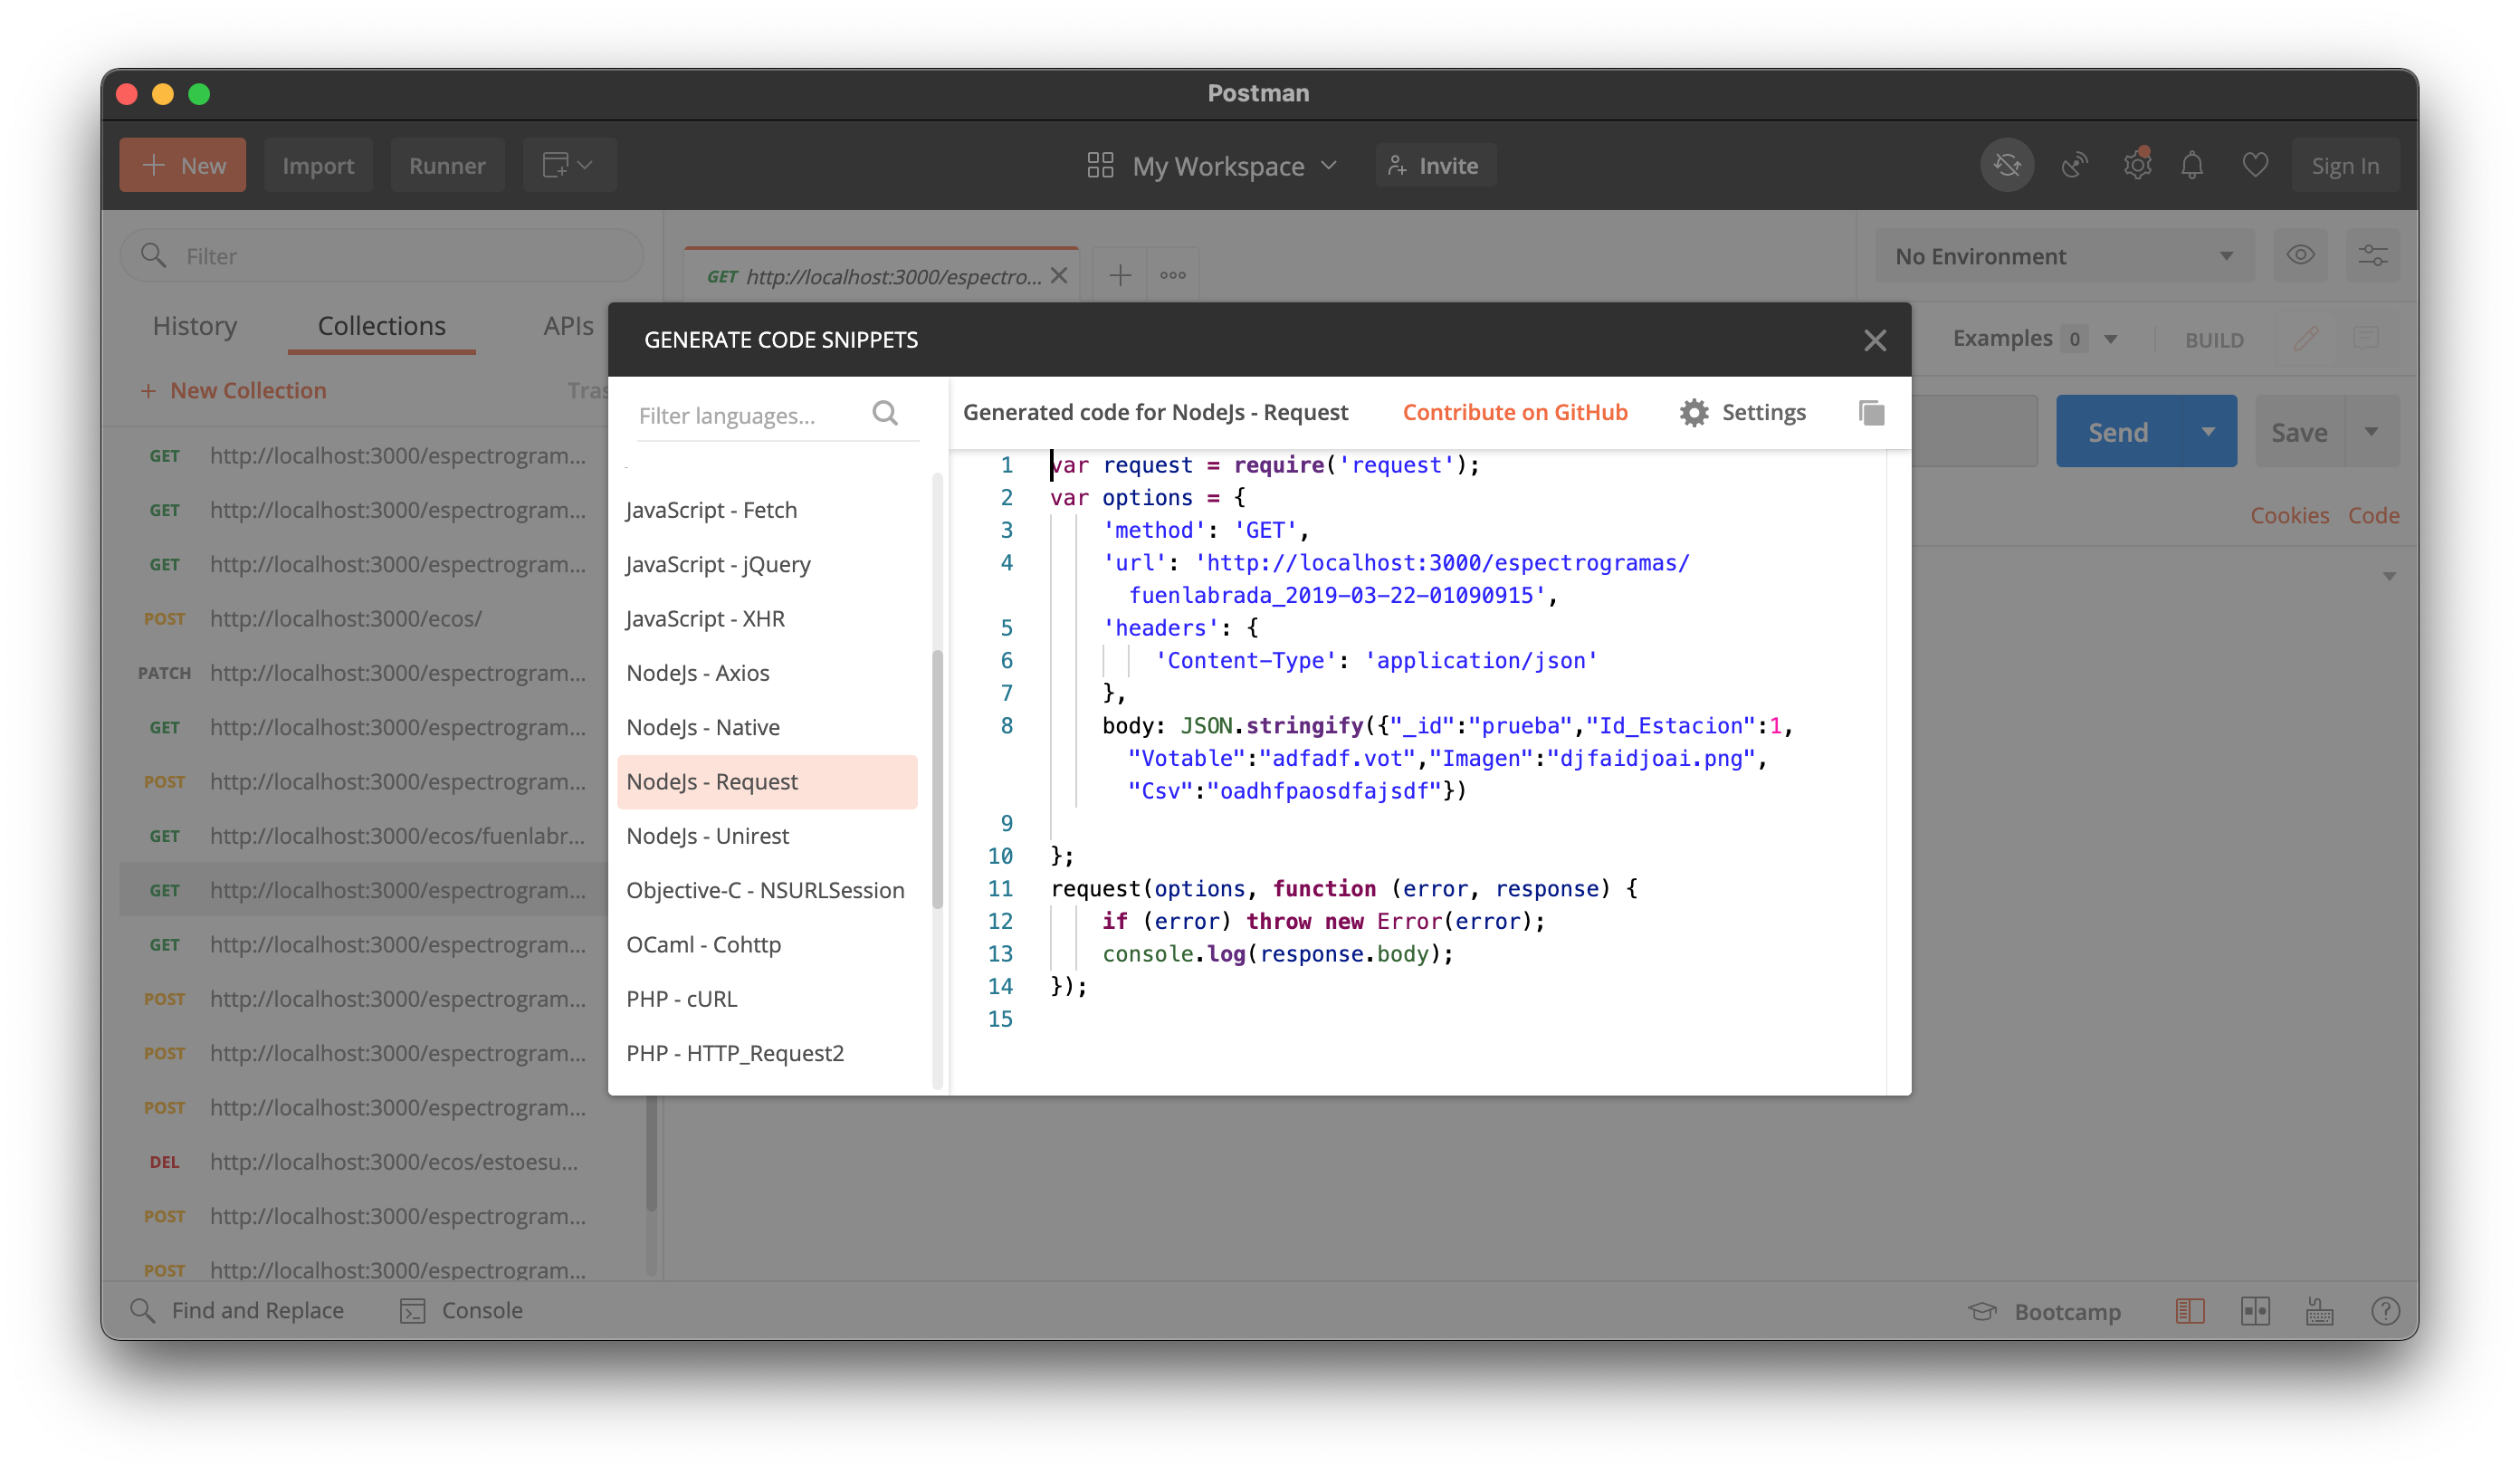
\includegraphics[width=\textwidth]{include/capturas/PostmanSnippet.png}
    \caption{Generador de código en Postman}
    \label{fig:postman_snippet}
\end{figure}

Otra característica interesante del programa es la capacidad de organizarse en entornos de trabajo, de esta forma si es necesario realizar test en más de un API Rest, además de poder definir variables y clasificarlas según los entornos de trabajo. También tiene una herramienta mediante la cual se puede generar automáticamente documentación de la API y exportar toda la configuración a un fichero JSON.


\subsection{Docker}

En cualquier proyecto de desarrollo de software que tenga un tamaño considerable siempre surge el mismo problema, el software que se ha desarrollado en una máquina tiene un rendimiento y funcionamiento diferentes al que tenía en la máquina del desarrollo.

\begin{figure}[H]
    \centering
    
\includegraphics[scale=0.05]{include/figuras/docker.png}
    \caption{Logo de Docker}
    \label{fig:docker_icon}
\end{figure}

\subsubsection{¿Qué es Docker?}
Se trata de una herramienta de virtualización pero a diferencia de las máquinas virtuales tradicionales es posible levantar el servicio de una forma mucho más rápida y en sistemas operativos mucho más eficientes. 
La idea principal es la de crear contenedores portables y ligeros de aplicaciones de software con la posibilidad de ejecutarse en cualquier dispositivo que tenga Docker instalado sin importar que sistema operativo esté funcionando \cite{docker}.

\subsubsection{Elementos básicos}
Docker se compone de tres elementos básicos

\begin{itemize}
    \item \textbf{Contenedor}: contiene todas las herramientas necesarias para el correcto funcionamiento de una aplicación sin necesidad de repositorios externos. Cada contenedor es una plataforma con sus propias directivas de seguridad y aislada del resto de la máquina.
    \item \textbf{Imagen Docker}: la imagen de docker se puede ver como un sistema operativo mínimo con aplicaciones instaladas (Por ejemplo un sistema operativo RedHat con MySQL instalado). A partir de una base se pueden añadir más elementos que sean necesarios en otro equipo donde se vaya a utilizar la imagen. Docker además proporciona herramientas sencillas mediantes las cuales mantener las imágenes actualizadas.
    \item \textbf{Docker Hub}: es el lugar donde se almacenan las imágenes creadas por otros usuarios de tal forma que cualquiera pueda utilizarlas. Existen repositorios públicos en los que todo el mundo puede utilizar las imágenes y repositorios privados en los cuales es necesario comprar las imágenes que se vayan a usar. Con estos registros es muy sencillo desarrollar nuevas imágenes utilizándolos como plantilla en la que añadir nuevos componentes.
\end{itemize}

\subsubsection{Funcionamiento}

Docker incluye una interfaz gráfica como se muestra en la figura \ref{fig:dockerUI} para gestionar las imágenes y contenedores que existen en el equipo además de realizar los cambios necesarios para crear nuestra propia imagen.

\begin{figure}[H]
    \centering
    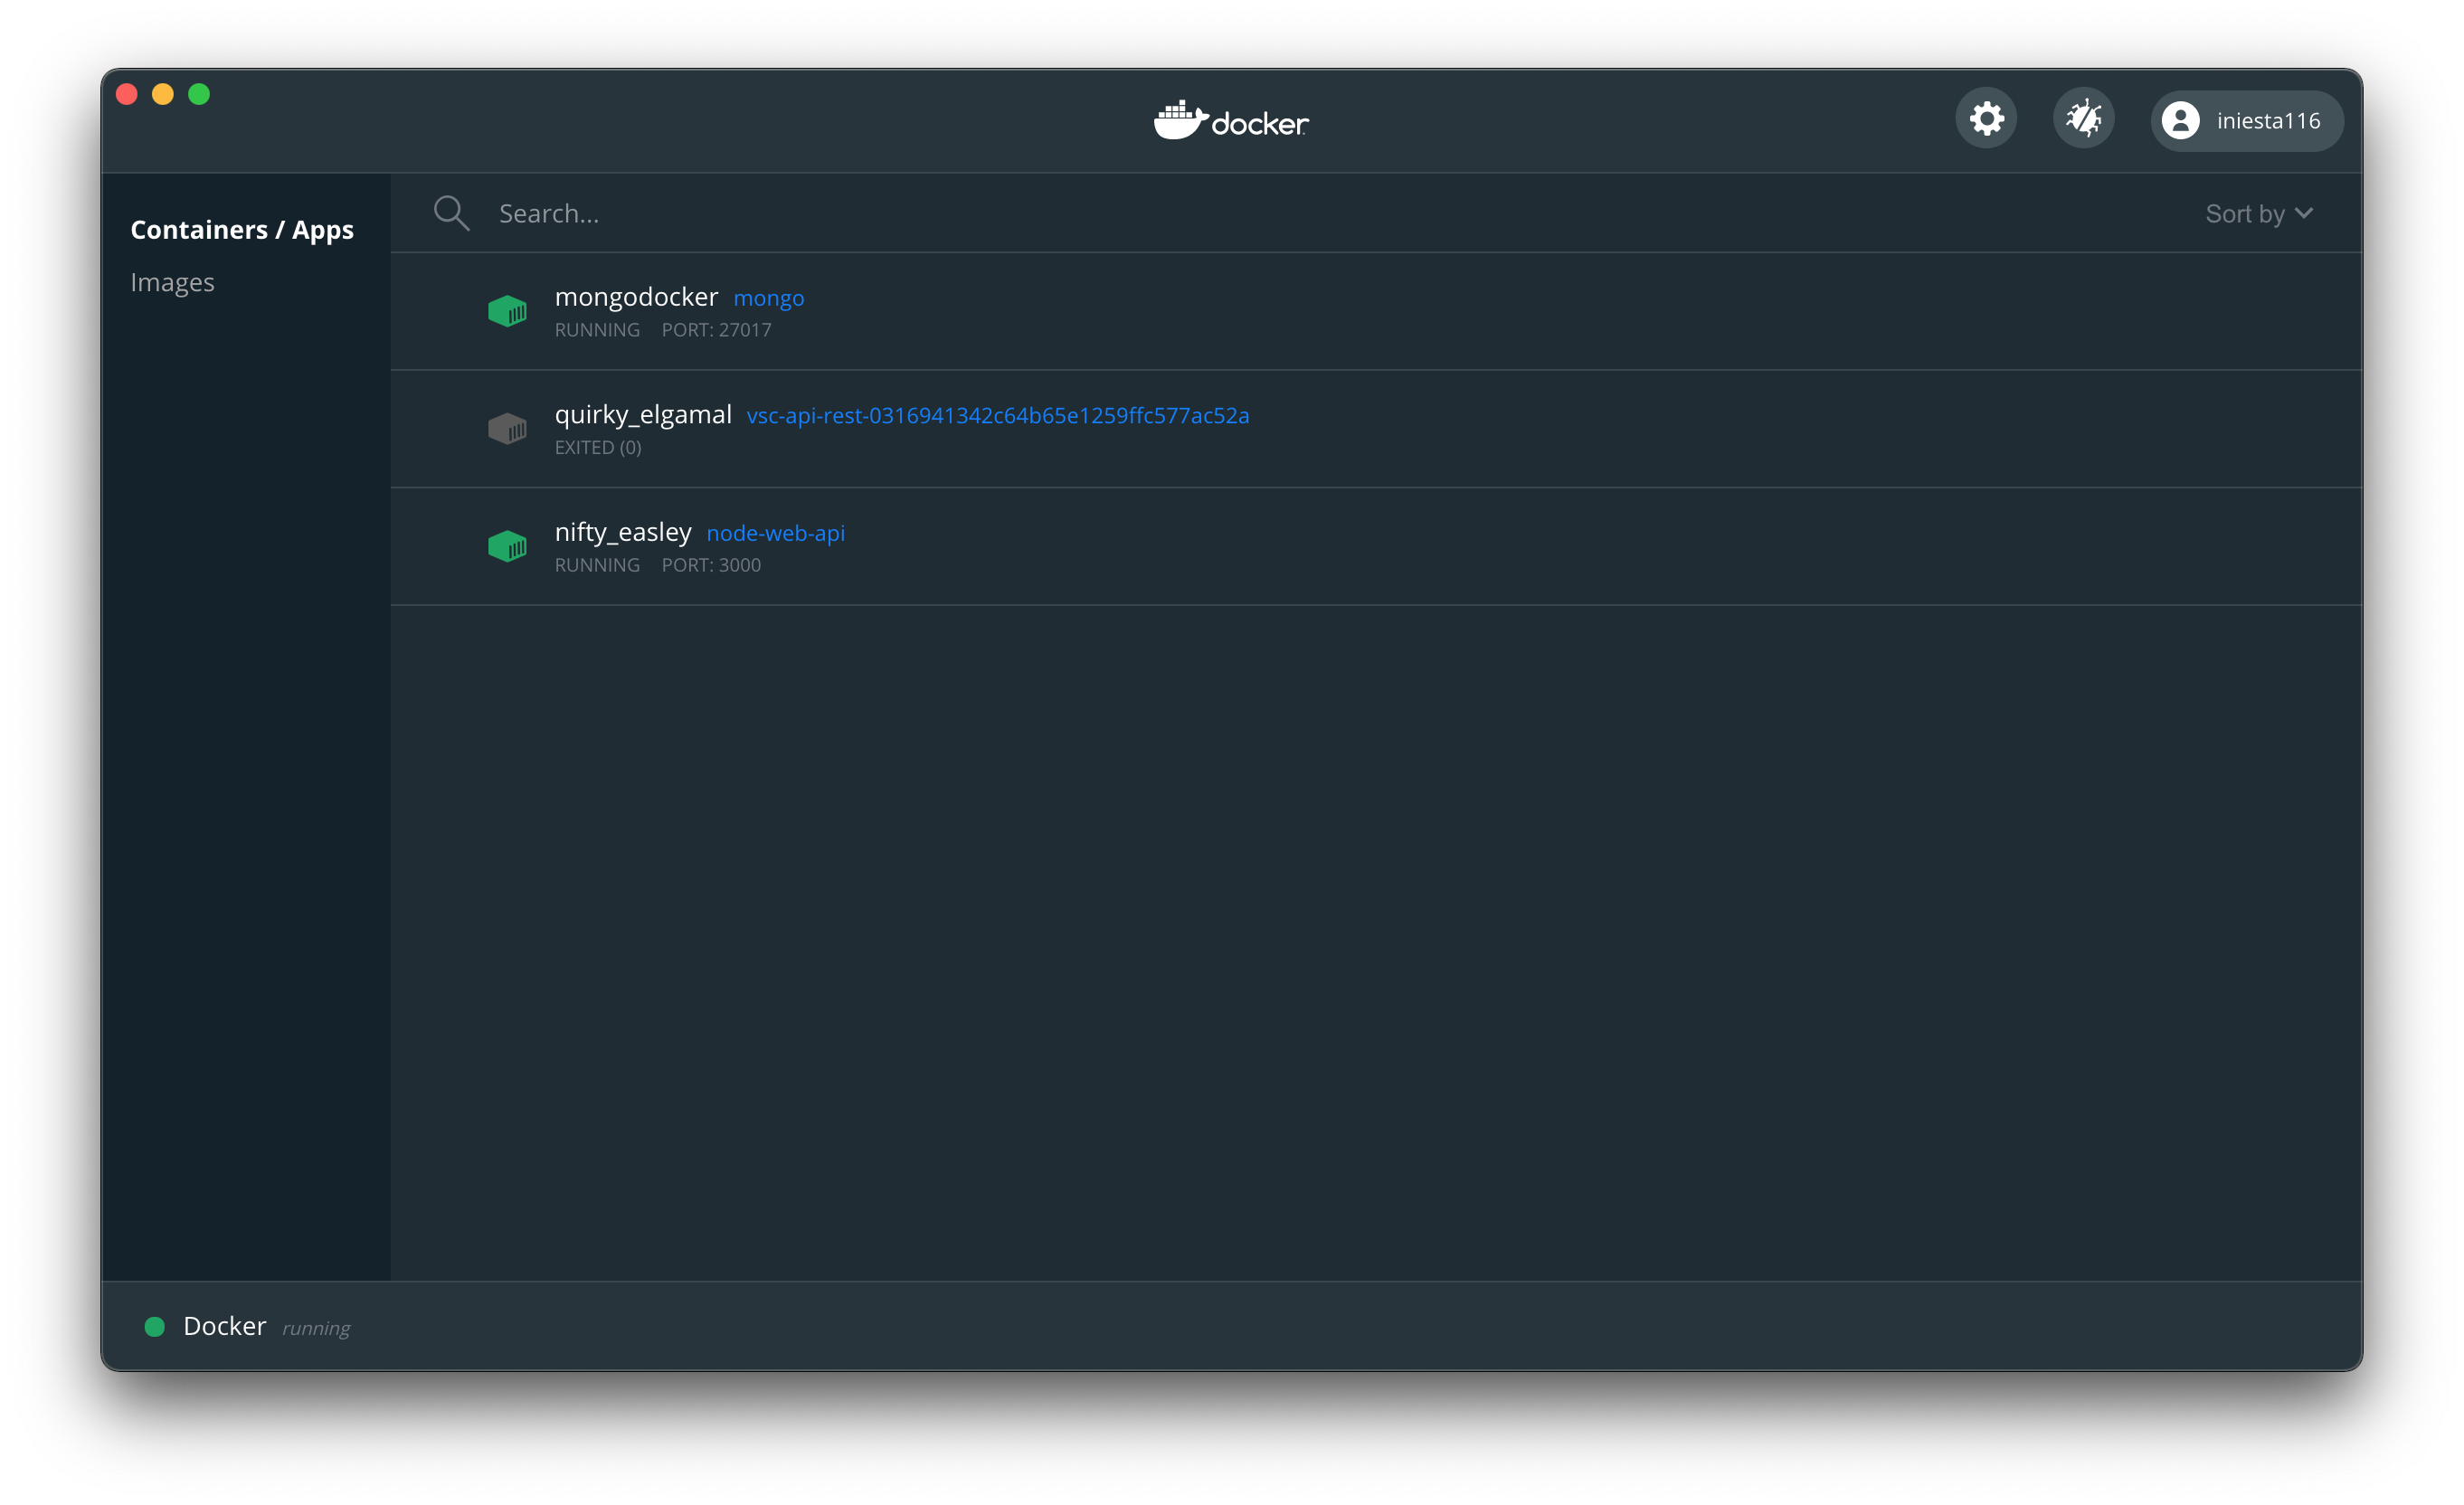
\includegraphics[scale=0.3]{include/capturas/DockerUI.png}
    \caption{Interfaz gráfica de Docker}
    \label{fig:dockerUI}
\end{figure}

Partiendo del ejemplo de una aplicación web, ésta necesita diferentes tipos de software para poder ser desarrollada y desplegada (spring, MySQL, Tomcat, Maven...). 

Docker permite introducir todo ese software dentro de un contenedor todas las herramientas que necesite la aplicación además de la propia aplicación. De esta forma, puedo transportar el contenedor a cualquier tipo de máquina (servidor, ordenador pórtatil, Raspberry PI, etc) que tenga instalado Docker y directamente ejecutar la aplicación sin necesidad de realizar instalaciones complementarias, ejecutar ninguna herramienta más o comprobar compatibilidades.

Cada vez que se vaya a ejecutar el contenedor serán necesarias tanto la imagen base como las nuevas 'capas' que se han añadido. Docker automáticamente se encarga de acoplar la base, la imagen y las distintas capas para levantar el entorno deseado sobre el que poder trabajar. 

\begin{figure}[H]
    \centering
    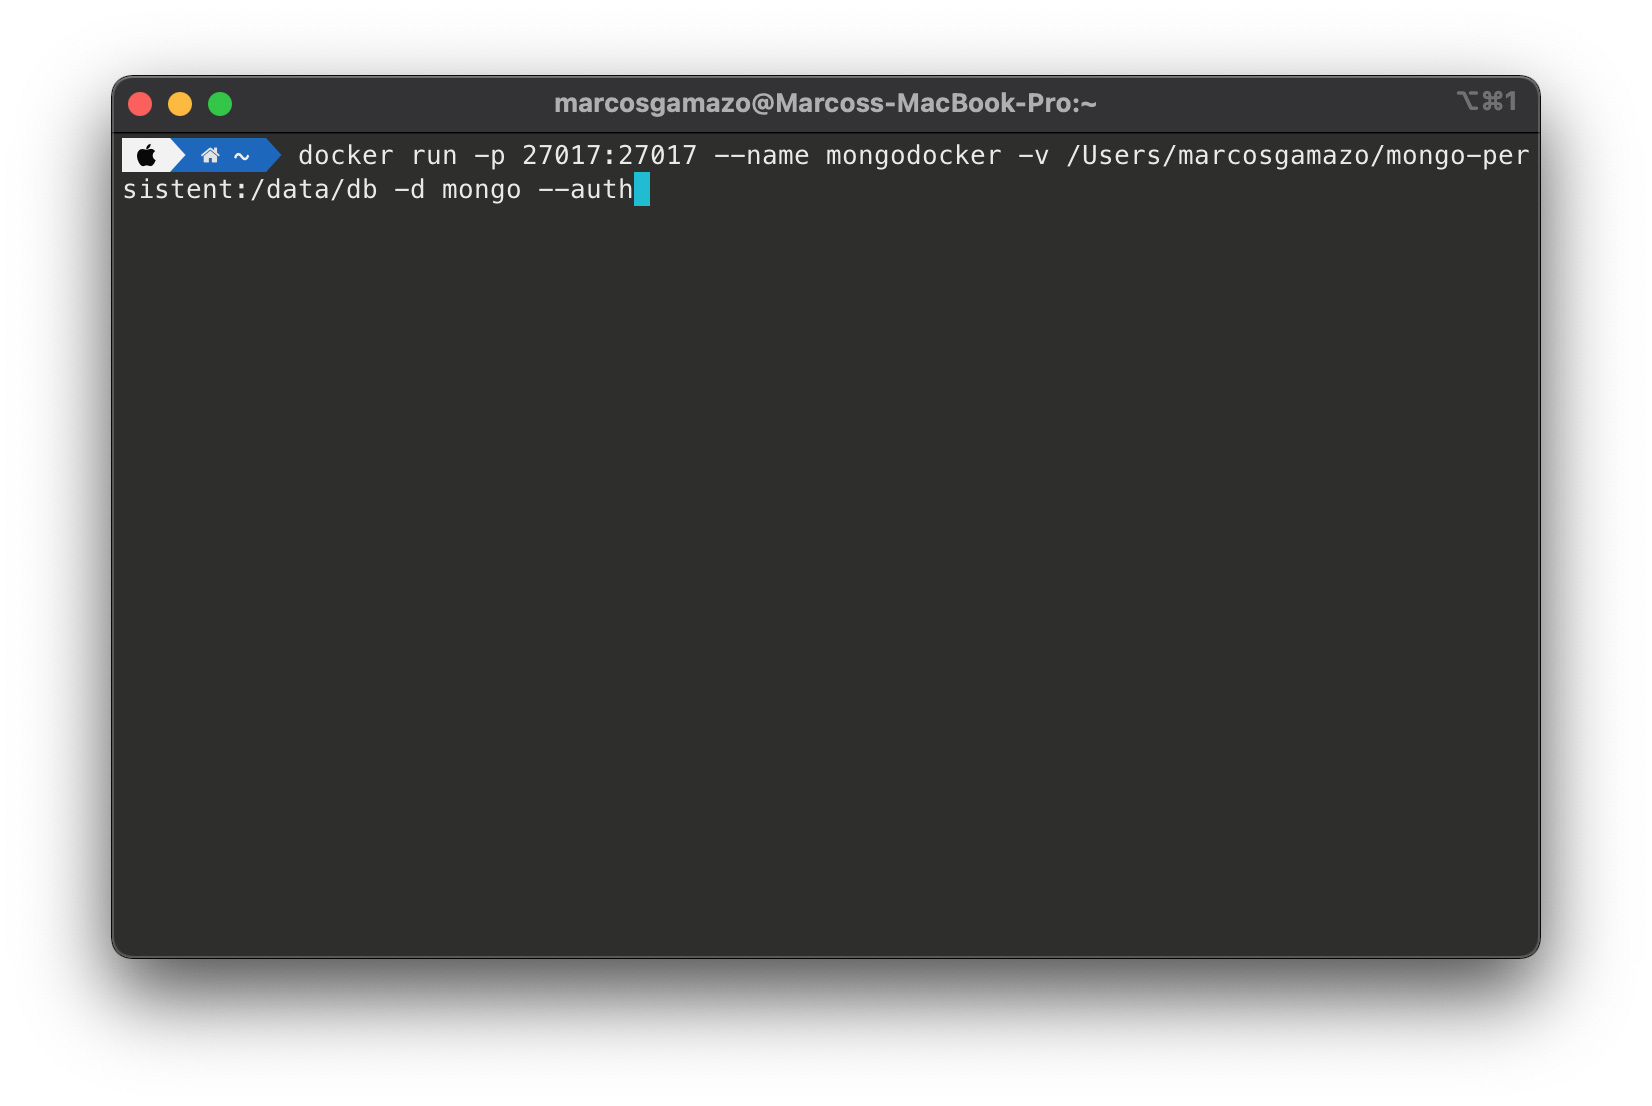
\includegraphics[width=0.5\textwidth]{include/capturas/dockerRun.png}
    \caption{Inicio de un contenedor docker}
    \label{fig:docker_run}
\end{figure}

Esto se puede hacer de manera muy sencilla mediante un terminal \cite{basicDocker} y un comando como se ve en la figura \ref{fig:docker_run} en la que se realiza un despliegue de una imagen con MongoDB sobre la que se ha desarrollado la base de datos del proyecto.

\subsubsection{Principales características}
\begin{itemize}
    \item Autogestión de los contenedores.
    \item Posibilidad de desplegar múltiples contenedores en un mismo equipo.
    \item Fiabilidad.
    \item Contenedores ligeros que simplifican la labor de almacenamiento, transporte y despliegue.
    \item Capacidad de ejecutar una gran variedad de aplicaciones.
    \item Levantar los servicios es una operación muy rápida.
    \item La aplicación Docker es capaz de gestionar los recursos de la máquina para asignarlos a los distintos contenedores.
    \item Compartir las imágenes en Docker Hub.
\end{itemize}

\subsubsection{Tipos de despliegues}
Existen varias formas de desplegar un contenedor en Docker, la más sencilla es la que se muestra en la figura \ref{fig:docker_run} en la que se puede crear un contenedor mediante un solo comando. 

Otra forma de hacerlo es mediante un \textit{Dockerfile} como el que se muestra a continuación:

\begin{lstlisting}
FROM ubuntu:latest
MAINTAINER john doe 

RUN apt-get update
RUN apt-get install -y python python-pip wget
RUN pip install Flask

ADD hello.py /home/hello.py

WORKDIR /home
\end{lstlisting}

Su funcionamiento es muy sencillo, se crea un fichero de texto plano en el que se indica la imagen base a utilizar y posteriormente mediante mandatos de terminal se instalan las distintas herramientas a incluir en la imagen personalizada. Una vez generada la imagen con el comando docker build se puede desplegar el contenedor mediante la interfaz gráfica o mediante la terminal.

\textit{Docker compose} es una herramienta pensada para definir y correr aplicaciones con múltiples contenedores, se pueden definir los distintos servicios que van a formar la aplicación dentro del fichero \textit{docker-compose.yml} de forma que pueden correr juntas en un entorno aislado.

\vspace{.7cm}
\begin{lstlisting}
version: "3"
services:
  web:
    build: .
    ports:
    - '5000:5000'
    volumes:
    - .:/code
    - logvolume01:/var/log
    links:
    - redis
  redis:
    image: redis
    volumes:
      logvolume01: {}
\end{lstlisting}

Una vez creado el fichero, el contenedor se puede levantar simplemente con el comando \textit{docker-compose up}.

\subsection{Rasa Framework}
\chapter{Resultados y conclusiones}

Resumen de resultados obtenidos en el TFG. Y conclusiones personales del estudiante sobre el trabajo realizado.
\chapter*{Anexo}
Este capítulo es opcional, y se escribirá de acuerdo con las indicaciones del Tutor. 


\section{Ejemplo de código en python}
\begin{lstlisting}[style=Python]
# -*- coding: utf-8 -*-
import sympy as sy
from sympy.abc import x
\end{lstlisting}

\section{Ejemplo de fórmula matemática}
$$e^{i \pi} + 1 = 0 $$




 

%\begin{thebibliography}{99}
\bibliographystyle{plain}
\bibliography{refs.bib}


\bibitem{Stream Generator} Citizen Science Lab. \textit{Contadores de Estrellas - Server Side - Echoes generator}.
\url{https://github.com/cslab-upm/Echoes-stream-generator}

\bibitem{INE} Insntituto Nacional de Estadística. \textit{Encuesta sobre Equipamiento y Uso de Tecnologías de Información y
Comunicación en los Hogares}
\url{https://www.ine.es/prensa/tich_2019.pdf}

\bibitem{Dialogflow} Carlos Denis \textit{Dialogflow: la herramienta de Google para la creación de Chatbots} \url{https://www.makingscience.com/blog/dialogflow-la-herramienta-de-google-para-la-creacion-de-chatbots/}

\bibitem{MicrosoftBotBuilder} Planeta Chatbot \textit{Información sobre desarrollo de bots de Microsoft} \url{https://planetachatbot.com/informacion-para-articulo-de-bots-de-microsoft-943a25eddd5}

\bibitem{ibmWatson} Rodolfo de Juana \textit{IBM Watson: casi todo lo que tienes que saber} \url{https://www.muycomputerpro.com/2019/09/24/ibm-watson-casi-todo-lo-que-tienes-que-saber}.

\bibitem{chatbotAI} Ahmad Faizal B H \textit{Chatbot} \url{https://github.com/ahmadfaizalbh/Chatbot}

\end{thebibliography}

%\begin{thebibliography}{99}
\bibliographystyle{plain}
\bibliography{refs.bib}


\bibitem{Stream Generator} Citizen Science Lab. \textit{Contadores de Estrellas - Server Side - Echoes generator}.
\url{https://github.com/cslab-upm/Echoes-stream-generator}

\bibitem{INE} Insntituto Nacional de Estadística. \textit{Encuesta sobre Equipamiento y Uso de Tecnologías de Información y
Comunicación en los Hogares}
\url{https://www.ine.es/prensa/tich_2019.pdf}

\bibitem{Dialogflow} Carlos Denis \textit{Dialogflow: la herramienta de Google para la creación de Chatbots} \url{https://www.makingscience.com/blog/dialogflow-la-herramienta-de-google-para-la-creacion-de-chatbots/}

\bibitem{MicrosoftBotBuilder} Planeta Chatbot \textit{Información sobre desarrollo de bots de Microsoft} \url{https://planetachatbot.com/informacion-para-articulo-de-bots-de-microsoft-943a25eddd5}

\bibitem{ibmWatson} Rodolfo de Juana \textit{IBM Watson: casi todo lo que tienes que saber} \url{https://www.muycomputerpro.com/2019/09/24/ibm-watson-casi-todo-lo-que-tienes-que-saber}.

\bibitem{chatbotAI} Ahmad Faizal B H \textit{Chatbot} \url{https://github.com/ahmadfaizalbh/Chatbot}

\end{thebibliography}


\bibliographystyle{ieeetr}
%\bibliographystyle{apalike}
\addcontentsline{toc}{chapter}{Bibliografía}
\bibliography{bibliographyfile}
\nocite{*} %SI QUEREMOS PONER TODAS LAS CITAS INCLUSO SI NO ESTAN CITADAS
%%-----------------------------------------------
%% Anexos
\appendix
\clearpage 
\addcontentsline{toc}{chapter}{Anexo}
\chapter*{Anexo}
Este capítulo es opcional, y se escribirá de acuerdo con las indicaciones del Tutor. 


\section{Ejemplo de código en python}
\begin{lstlisting}[style=Python]
# -*- coding: utf-8 -*-
import sympy as sy
from sympy.abc import x
\end{lstlisting}

\section{Ejemplo de fórmula matemática}
$$e^{i \pi} + 1 = 0 $$




 
%%---------------------------------------------------------
\end{document}
